\begingroup
\fontencoding{T5}\selectfont
\section{Hiện thực Hệ thống}

Chương này mô tả chi tiết việc hiện thực Hệ thống Quản lý Thư viện Trực tuyến BkLib. Đầu tiên, chương giới thiệu về công nghệ và các thành phần kiến trúc vận hành nền tảng, tiếp theo là chi tiết từng mô-đun bao gồm cả giao diện người dùng và hiện thực kỹ thuật cốt lõi (dịch vụ backend, logic nghiệp vụ và các đoạn mã nguồn tiêu biểu).

% =========================================================================
% SECTION 5.1: TECHNOLOGY STACK
% =========================================================================
\subsection{Tập công nghệ (Technology Stack)}

\subsubsection{Front-end: React.js và Vite}
React.js đảm nhận tầng giao diện của thư viện trực tuyến, xây dựng các giao diện tương tác cho việc tìm kiếm sách, duyệt danh mục và trò chuyện với trợ lý AI. Vite được sử dụng làm công cụ đóng gói và máy chủ phát triển giúp khởi động nhanh, hỗ trợ HMR (Hot Module Replacement) và tối ưu hóa việc biên dịch sản phẩm. Phía máy khách, các thành phần xử lý việc hiển thị kết quả tìm kiếm (kết hợp tô sáng từ khóa và khớp ngữ nghĩa), quản lý trạng thái người dùng (cache, cập nhật lạc quan) và tích hợp SDK chatbot/trợ lý AI (phản hồi dạng streaming, trạng thái hội thoại).
\begin{figure}[htbp]
    \centering
    
\includegraphics[width=0.4\textwidth]{Images/react_vite.png}
\end{figure}

\subsubsection{Back-end: Node.js và Express}
Node.js + Express cung cấp các REST API cốt lõi cho việc quản lý danh mục sách, tài khoản người dùng và quản trị phiên làm việc. Máy chủ điều phối việc định tuyến yêu cầu, xác thực, phân quyền RBAC, các giao dịch PostgreSQL thông qua Prisma và ủy quyền các tác vụ AI (tạo vector nhúng, tóm tắt, truy vấn RAG) cho dịch vụ AI chuyên biệt. Máy chủ cung cấp các điểm cuối API tiêu chuẩn cho tìm kiếm, gợi ý và tích hợp webhook (ví dụ: làm giàu dữ liệu tả từ Open Library).
\begin{figure}[htbp]
    \centering
    
\includegraphics[width=0.4\textwidth]{Images/node_express.jpg}
\end{figure}

\subsubsection{Dịch vụ AI Microservice Chuyên biệt: Python và FastAPI}
Dịch vụ microservice độc lập được triển khai bằng Python + FastAPI tận dụng các thư viện Xử lý Ngôn ngữ Tự nhiên (NLP) và Mã nguồn Mở Machine Learning (transformers, sentence-transformers, SDK client của các nhà cung cấp LLM). Nhiệm vụ chính bao gồm tạo vector nhúng, tóm tắt tài liệu, trả lời câu hỏi dựa trên RAG và các đường ống xử lý prompt (chia đoạn, xếp hạng lại). FastAPI là lựa chọn lý tưởng cho các điểm cuối API bất đồng bộ độ trễ thấp và có thể mở rộng linh hoạt theo tải công việc.
\begin{figure}[htbp]
    \centering
    
\includegraphics[width=0.4\textwidth]{Images/fastapi.png}
\end{figure}

\subsubsection{ORM: Prisma}
Prisma (TypeScript) được sử dụng để định nghĩa lược đồ cơ sở dữ liệu, tạo các truy vấn an toàn kiểu dữ liệu và quản lý các migration của PostgreSQL. Prisma duy trì tính an toàn kiểu end-to-end giữa ứng dụng Node và tầng cơ sở dữ liệu, đơn giản hóa các truy vấn liên quan đến lượt mượn, nhật ký giao dịch và dữ liệu tả danh mục đồng thời hỗ trợ giao dịch ACID cho tính nhất quán dữ liệu.
\begin{figure}[htbp]
    \centering
    
\includegraphics[width=0.4\textwidth]{Images/prisma.png}
\end{figure}

\subsubsection{Cơ sở Dữ liệu Quan hệ: PostgreSQL}
PostgreSQL đóng vai trò là kho lưu trữ quan hệ chính cho các bản ghi sách, hồ sơ người dùng, giao dịch mượn trả và dữ liệu tả hệ thống. Ưu điểm chính bao gồm sự tuân thủ nghiêm ngặt chuẩn ACID cho quy trình mượn trả, hỗ trợ JSONB nâng cao cho dữ liệu tả linh hoạt, chỉ mục từ khóa toàn văn (full-text search) và khả năng mở rộng ngang qua nhân bản và phân mảnh.
\begin{figure}[htbp]
    \centering
    
\includegraphics[width=0.4\textwidth]{Images/postgresql.jpg}
\end{figure}

\subsubsection{Kho Lưu trữ Vector và Embeddings: pgvector}
Các vector nhúng văn bản cho nội dung sách (toàn văn, tóm tắt) được lưu trữ trong `pgvector` (mở rộng vector cho PostgreSQL) hoặc cơ sở dữ liệu vector chuyên dụng. Kho vector thực hiện các phép tìm kiếm láng giềng gần nhất (độ tương đồng cosine) để phục vụ tìm kiếm ngữ nghĩa, truy xuất ngữ cảnh cho đường ống RAG và tính năng gợi ý "sách tương tự", ánh xạ kết quả vector trực tiếp đến ID tài liệu gốc.
\begin{figure}[htbp]
    \centering
    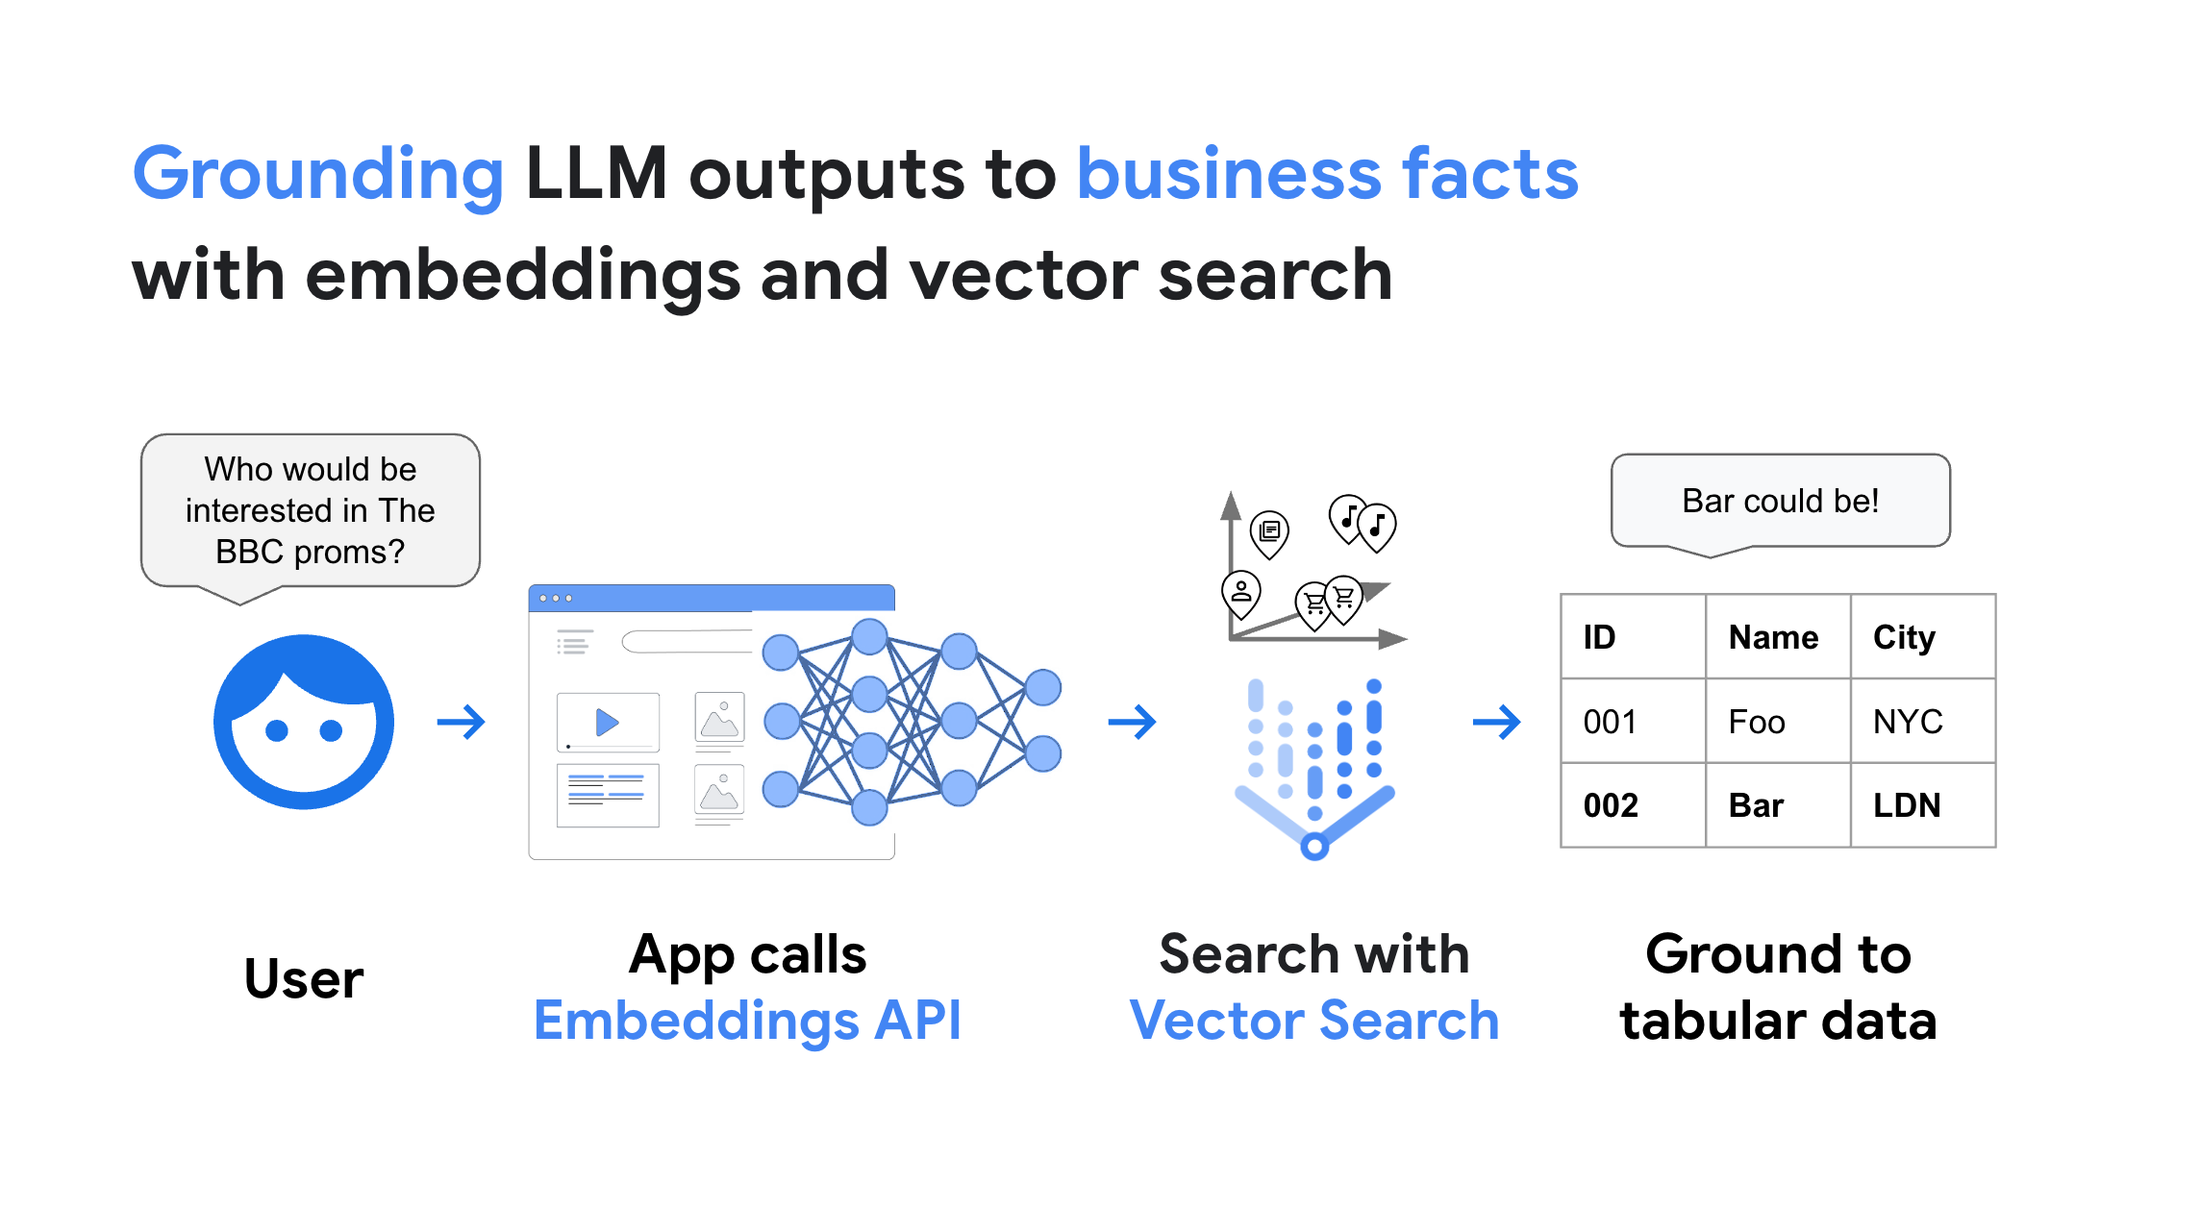
\includegraphics[width=0.5\textwidth]{Images/EmbeddingsAPI.png}
\end{figure}

\subsubsection{Chiến lược Tìm kiếm Kết hợp (Hybrid Search)}
Chiến lược tìm kiếm kết hợp phối hợp giữa: 1) tìm kiếm từ khóa toàn văn trên PostgreSQL để khớp dữ liệu tả chính xác; và 2) tìm kiếm tương đồng vector qua pgvector để truy xuất ngữ nghĩa và khớp ngữ cảnh. Kết quả được gộp và xếp hạng lại (dựa trên điểm độ liên quan, độ phổ biến và ngữ cảnh người dùng) trước khi trả về giao diện máy khách.

\subsubsection{An ninh và Xác thực: JWT, RBAC và OTP}
Hệ thống sử dụng JSON Web Token (JWT) cho quản lý phiên làm việc và refresh token cho sự duy trì an toàn. Kiểm soát Truy cập Dựa trên Vai trò (RBAC) áp dụng các quyền chi tiết (Admin, Thủ thư, Độc giả) được xác thực tại gateway API và các điểm cuối endpoints. Mật khẩu Một lần (OTP qua email/SMS) bảo vệ xác thực đa yếu tố cho các thao tác nhạy cảm. Các biện pháp bổ sung bao gồm mã hóa HTTPS/TLS, giới hạn tần suất gửi yêu cầu (rate limiting) và ghi nhật ký kiểm toán toàn diện.

\subsubsection{Tích hợp Bên ngoài: Open Library, Google Books và Nodemailer}
API Open Library và Google Books tự động hóa việc lấy dữ liệu tả, ảnh bìa và dữ liệu xuất bản qua mã ISBN. Một đường ống ETL tự động định kỳ đồng bộ dữ liệu danh mục. `Nodemailer` xử lý các thông báo giao dịch (nhắc hạn trả sách, đặt lại mật khẩu, cảnh báo hệ thống) với các mẫu HTML động và ghi nhật ký phân phối.
\begin{figure}[htbp]
    \centering
    
\includegraphics[width=0.3\textwidth]{Images/Google-play-book-icon.png}
\end{figure}

% =========================================================================
% SECTION 5.2: AUTHENTICATION MODULE
% =========================================================================
\subsection{Mô-đun Xác thực}

Mô-đun Xác thực đóng vai trò là cổng chính để truy cập hệ thống cho tất cả các vai trò người dùng trong hệ thống BkLib. Mô-đun thực thi xác minh danh tính an toàn, điều hướng truy cập dựa trên vai trò, đăng ký thành viên tự phục vụ, khôi phục mật khẩu đa bước và middleware phân quyền bằng JSON Web Token (JWT).

\subsubsection{Hiện thực Giao diện Người dùng}

\paragraph{Trang Đăng nhập}
Cổng truy cập chính cung cấp xác thực hợp nhất với các thẻ chuyển đổi vai trò.

\begin{figure}[H]
    \centering
    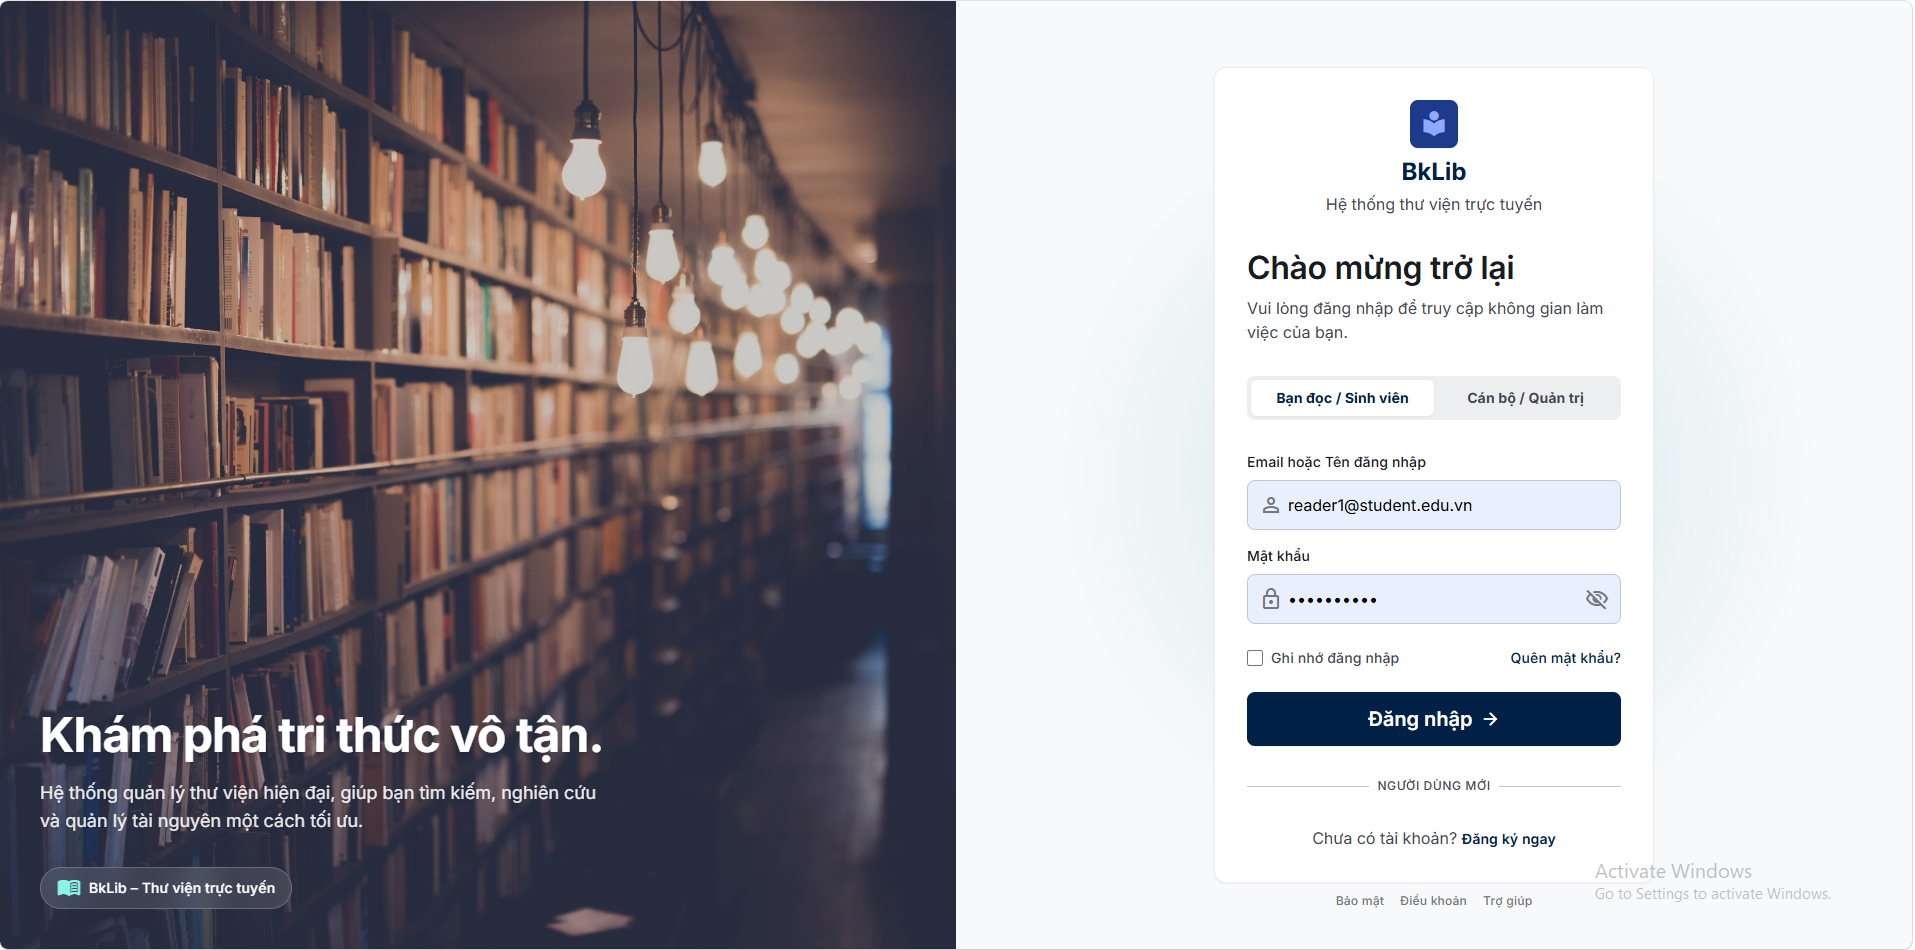
\includegraphics[width=0.95\linewidth]{Images/Auth_DangNhap.png}
    \vspace{10pt}
    \caption{Giao diện Đăng nhập BkLib}
    \label{fig:auth_login}
\end{figure}

\textbf{Bố cục \& Chức năng:} Thiết kế chia màn hình với hình ảnh thương hiệu ở bên trái và thẻ xác thực sạch sẽ ở bên phải. Bao gồm các tab lựa chọn vai trò ("Bạn đọc / Sinh viên" và "Cán bộ / Quản trị"), các trường nhập thông tin (email hoặc tên đăng nhập, mật khẩu có tùy chọn ẩn/hiện), hộp kiểm "Ghi nhớ đăng nhập", và các nút kích hoạt trực tiếp cho khôi phục mật khẩu ("Quên mật khẩu?") và đăng ký tài khoản. Sau khi xác thực, người dùng tự động được chuyển hướng về không gian làm việc tương ứng.

\paragraph{Trang Đăng ký}
Trang đăng ký tự phục vụ cho thành viên mới với tùy chọn chọn chi nhánh.

\begin{figure}[H]
    \centering
    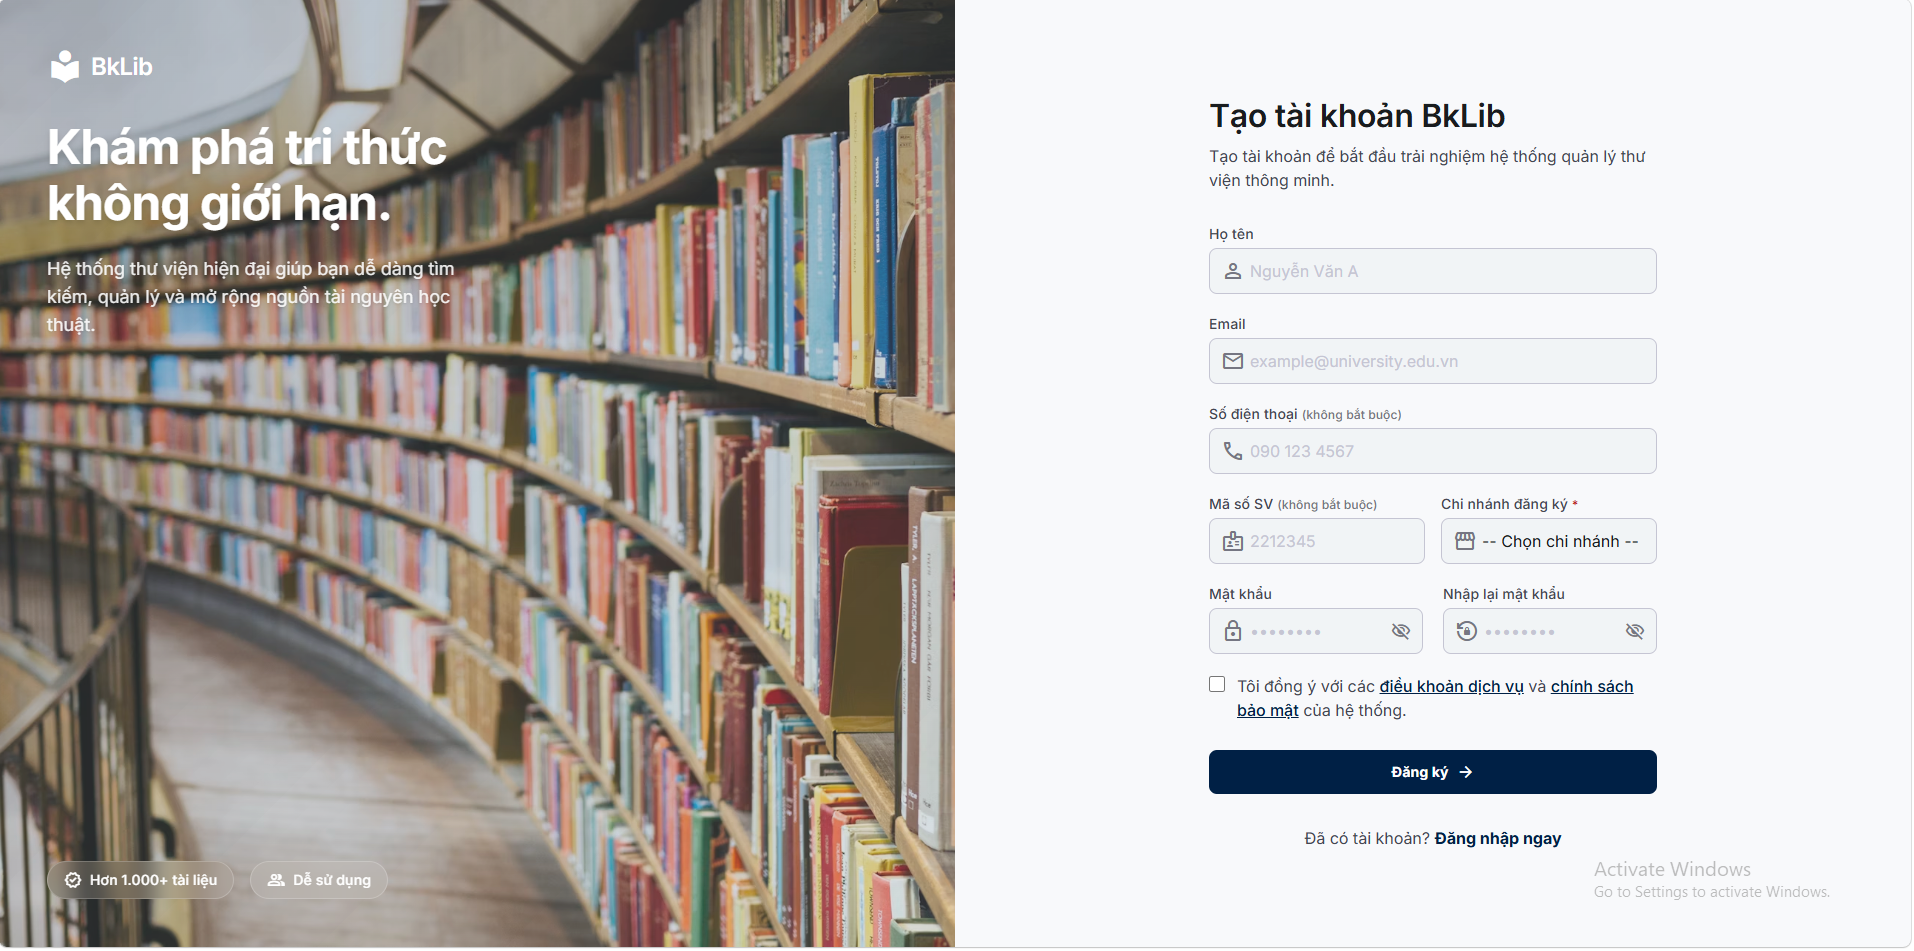
\includegraphics[width=0.95\linewidth]{Images/Auth_DangKy.png}
    \vspace{10pt}
    \caption{Giao diện Đăng ký Tài khoản BkLib}
    \label{fig:auth_register}
\end{figure}

\textbf{Bố cục \& Chức năng:} Biểu mẫu cấu trúc thu thập thông tin hồ sơ người dùng cơ bản, bao gồm Họ và Tên, Email, Số điện thoại (tùy chọn), Mã số Sinh viên ("Mã số SV" - tùy chọn) và Lựa chọn Chi nhánh ("Chi nhánh đăng ký"). Yêu cầu tạo mật khẩu với xác nhận khớp và đồng ý với điều khoản dịch vụ ("Điều khoản dịch vụ" và "Chính sách bảo mật") trước khi gửi yêu cầu đăng ký.

\paragraph{Quy trình Đặt lại Mật khẩu (Modal 3 bước)}
Cơ chế khôi phục mật khẩu tự phục vụ dạng modal sử dụng mã xác thực Email OTP 6 chữ số.

\begin{figure}[H]
    \centering
    \begin{subfigure}[b]{0.32\textwidth}
        \centering
        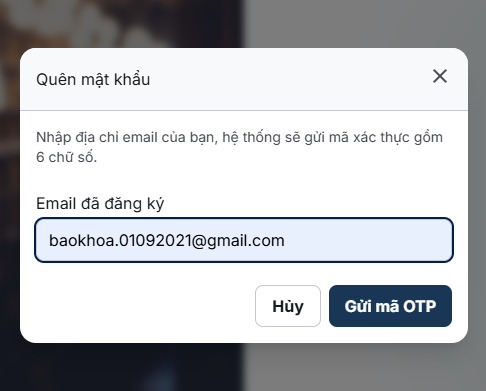
\includegraphics[width=\textwidth]{Images/Auth_QuenMatKhau_B1.png}
        \caption{Bước 1: Gửi Email}
        \label{fig:auth_reset_step1}
    \end{subfigure}
    \hfill
    \begin{subfigure}[b]{0.32\textwidth}
        \centering
        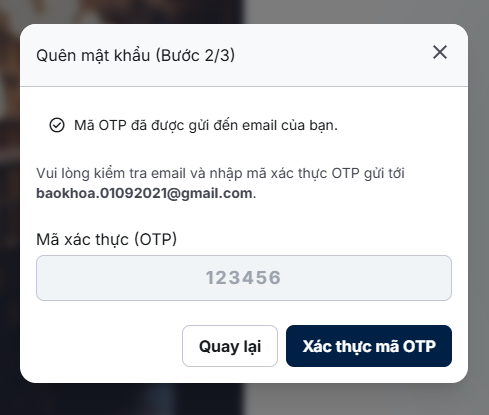
\includegraphics[width=\textwidth]{Images/Auth_QuenMatKhau_B2.png}
        \caption{Bước 2: Xác thực OTP}
        \label{fig:auth_reset_step2}
    \end{subfigure}
    \hfill
    \begin{subfigure}[b]{0.32\textwidth}
        \centering
        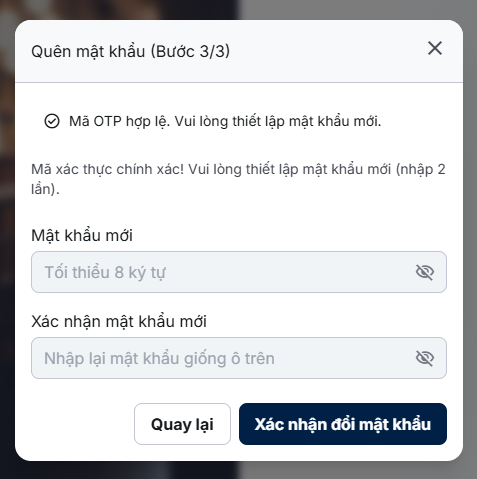
\includegraphics[width=\textwidth]{Images/Auth_QuenMatKhau_B3.png}
        \caption{Bước 3: Đặt lại Mật khẩu}
        \label{fig:auth_reset_step3}
    \end{subfigure}
    \vspace{10pt}
    \caption{Quy trình Modal 3 bước cho Khôi phục Mật khẩu}
    \label{fig:auth_forgot_password_flow}
\end{figure}

\textbf{Bố cục \& Chức năng:} Thực thi trong một hộp thoại modal đè lên gồm 3 giai đoạn tuần tự:
\begin{itemize}
    \item \textbf{Bước 1 (Yêu cầu OTP):} Người dùng nhập địa chỉ email đã đăng ký để hệ thống gửi mã xác thực 6 chữ số.
    \item \textbf{Bước 2 (Xác thực OTP):} Yêu cầu nhập mã 6 chữ số nhận được qua email, có phản hồi kiểm tra và nút quay lại.
    \item \textbf{Bước 3 (Cập nhật Mật khẩu):} Yêu cầu tạo và xác nhận mật khẩu mới (tối thiểu 8 ký tự) với biểu tượng con mắt để ẩn/hiện mật khẩu.
\end{itemize}

\subsubsection{Các Điểm sáng Hiện thực Kỹ thuật}

An ninh và bảo vệ các điểm cuối API được thực thi qua middleware sử dụng JSON Web Token (JWT) và hàm phân quyền vai trò bậc cao.

\begin{lstlisting}[caption={Middleware Xác thực và Phân quyền JWT (backend-express/src/middlewares/auth.middleware.ts)}, label={lst:auth_middleware}]
// Middleware verifing JWT access token from Authorization header
export const authenticate = (req: Request, res: Response, next: NextFunction): void => {
  const authHeader = req.headers.authorization;
  if (!authHeader || !authHeader.startsWith('Bearer ')) {
    res.status(401).json({ success: false, message: 'No authorization token provided' });
    return;
  }
  const token = authHeader.split(' ')[1];
  try {
    const decoded = jwt.verify(token, env.JWT_SECRET) as AuthPayload;
    req.user = decoded;
    next();
  } catch (err) {
    res.status(401).json({ success: false, message: 'Invalid or expired token' });
  }
};

// Middleware factory restricting access to specified roles
export const authorize = (...roles: Role[]) => {
  return (req: Request, res: Response, next: NextFunction): void => {
    if (!req.user || !roles.includes(req.user.role)) {
      res.status(403).json({ success: false, message: 'Access denied' });
      return;
    }
    next();
  };
};
\end{lstlisting}

% =========================================================================
% SECTION 5.3: READER MODULE
% =========================================================================
\subsection{Mô-đun Độc giả}

Mô-đun Độc giả cung cấp các khả năng tự phục vụ cho bạn đọc thư viện. Cho phép độc giả đã xác thực duyệt danh mục, thực hiện tìm kiếm bằng AI ngữ nghĩa, theo dõi và gia hạn lượt mượn, giám sát vị trí hàng chờ đặt chỗ, xem lịch sử giao dịch mượn trả và tương tác với widget trợ lý ảo.

\subsubsection{Hiện thực Giao diện Người dùng}

\paragraph{Trang chủ}
Bảng điều khiển trung tâm cá nhân hóa hiển thị sau khi độc giả đăng nhập, đóng vai trò là trung tâm vận hành cho các hoạt động của bạn đọc.

\begin{figure}[H]
    \centering
    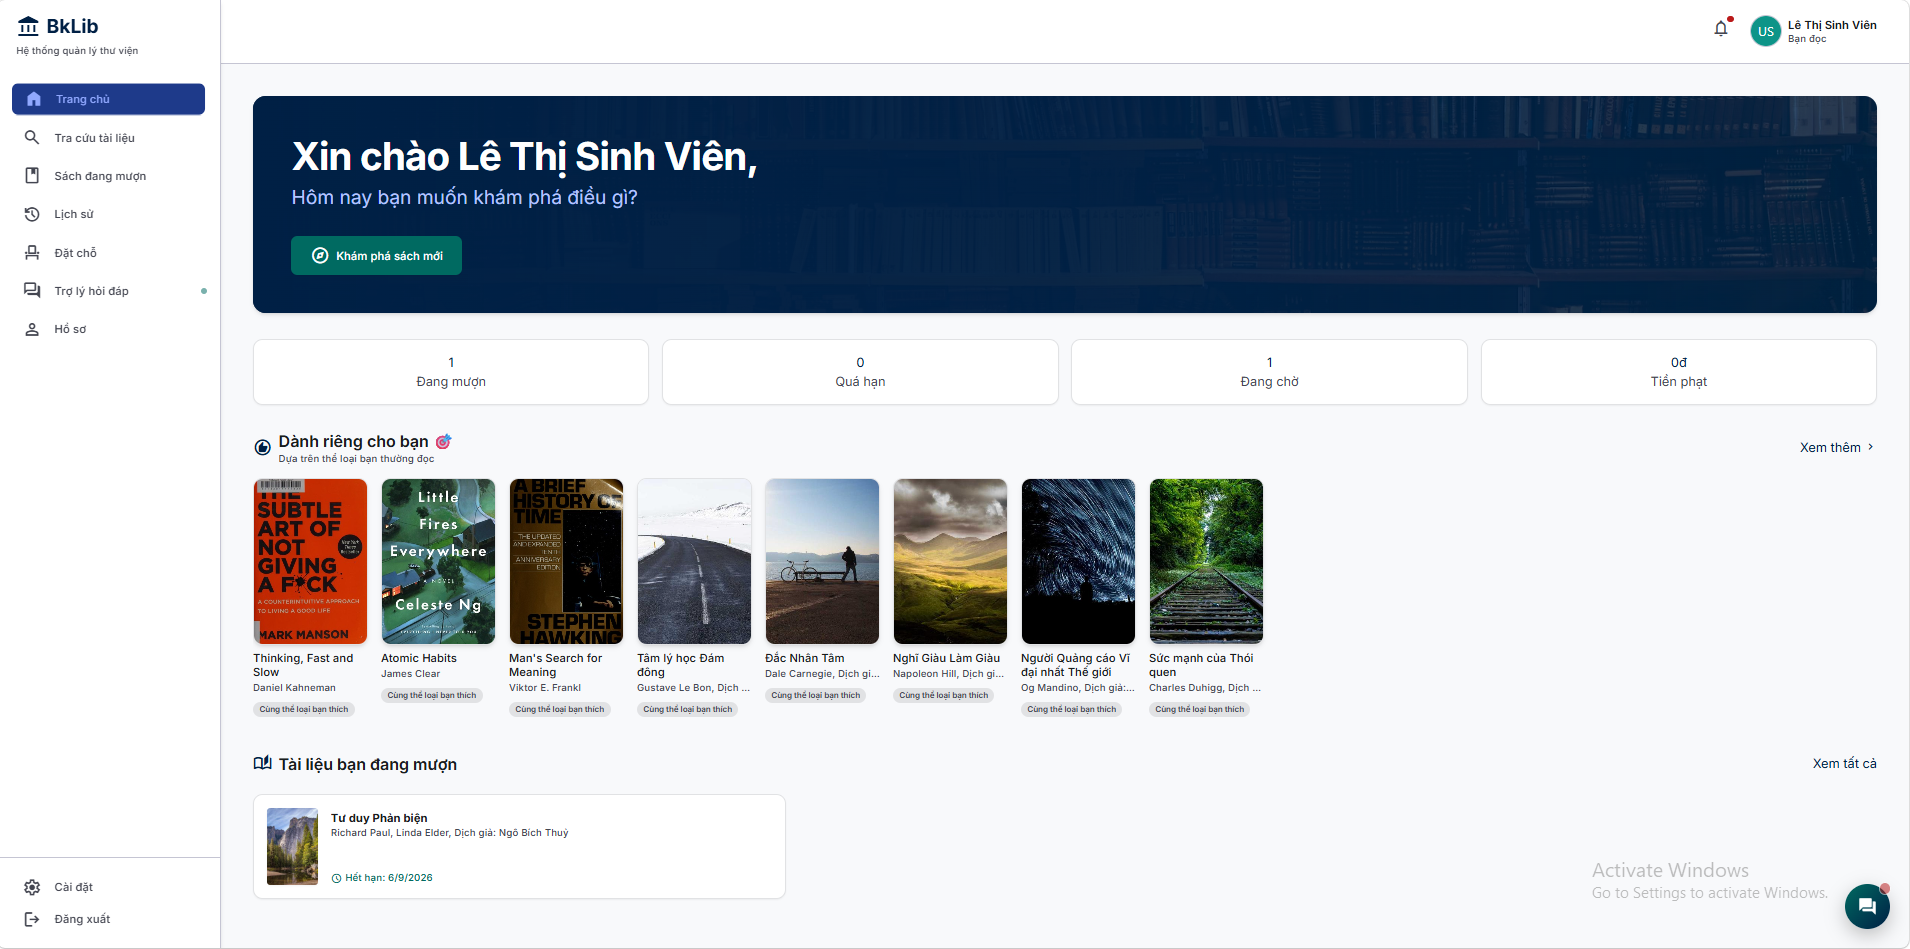
\includegraphics[width=0.95\linewidth]{Images/Reader_TrangChu.png}
    \vspace{10pt}
    \caption{Giao diện Trang chủ Mô-đun Độc giả}
    \label{fig:reader_homepage}
\end{figure}

\textbf{Bố cục \& Chức năng:} Bao gồm thanh điều hướng bên trái đáp ứng, trung tâm thông báo phía trên, các thẻ tóm tắt chỉ số chính (sách đang mượn, tài liệu quá hạn, số lượt đặt chỗ, số dư tiền phạt) và các thẻ truy cập nhanh cho các sách đang mượn với chỉ báo thời hạn trả theo thời gian thực.

\paragraph{Trang Tra cứu Danh mục}
Giao diện khám phá, lọc đa tiêu chí và duyệt danh mục tài nguyên thư viện.

\begin{figure}[H]
    \centering
    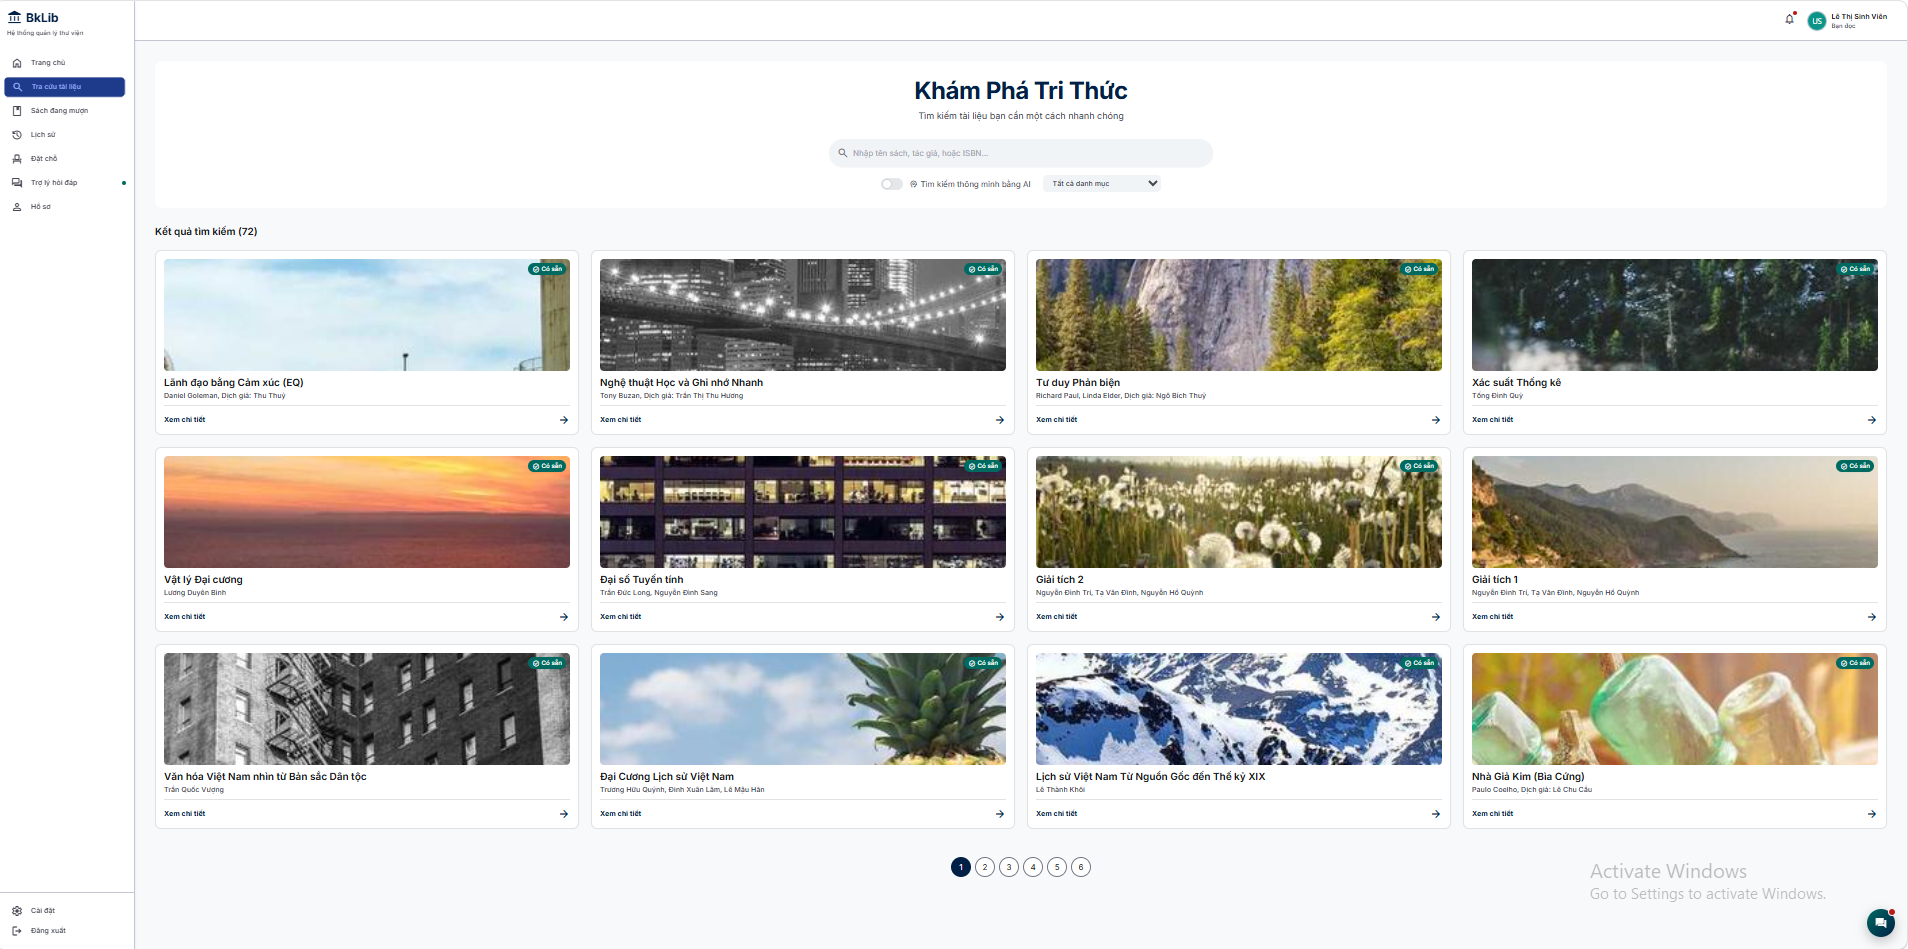
\includegraphics[width=0.95\linewidth]{Images/Reader_TraCuu.png}
    \vspace{10pt}
    \caption{Giao diện Tra cứu Danh mục}
    \label{fig:reader_search}
\end{figure}

\textbf{Bố cục \& Chức năng:} Tích hợp thanh tìm kiếm từ khóa nâng cao với bộ lọc thể loại và tính khả dụng theo chi nhánh. Độc giả có thể xem ảnh bìa, dữ liệu tả (tác giả, nhà xuất bản, ISBN), trạng thái khả dụng thực tế và thực hiện đặt chỗ trực tiếp từ các thẻ kết quả tìm kiếm.

\paragraph{Trang Quản lý Sách Đang Mượn}
Giao diện chuyên biệt cho phép độc giả theo dõi vòng đời lượt mượn và kích hoạt gia hạn mượn sách trực tuyến.

\begin{figure}[H]
    \centering
    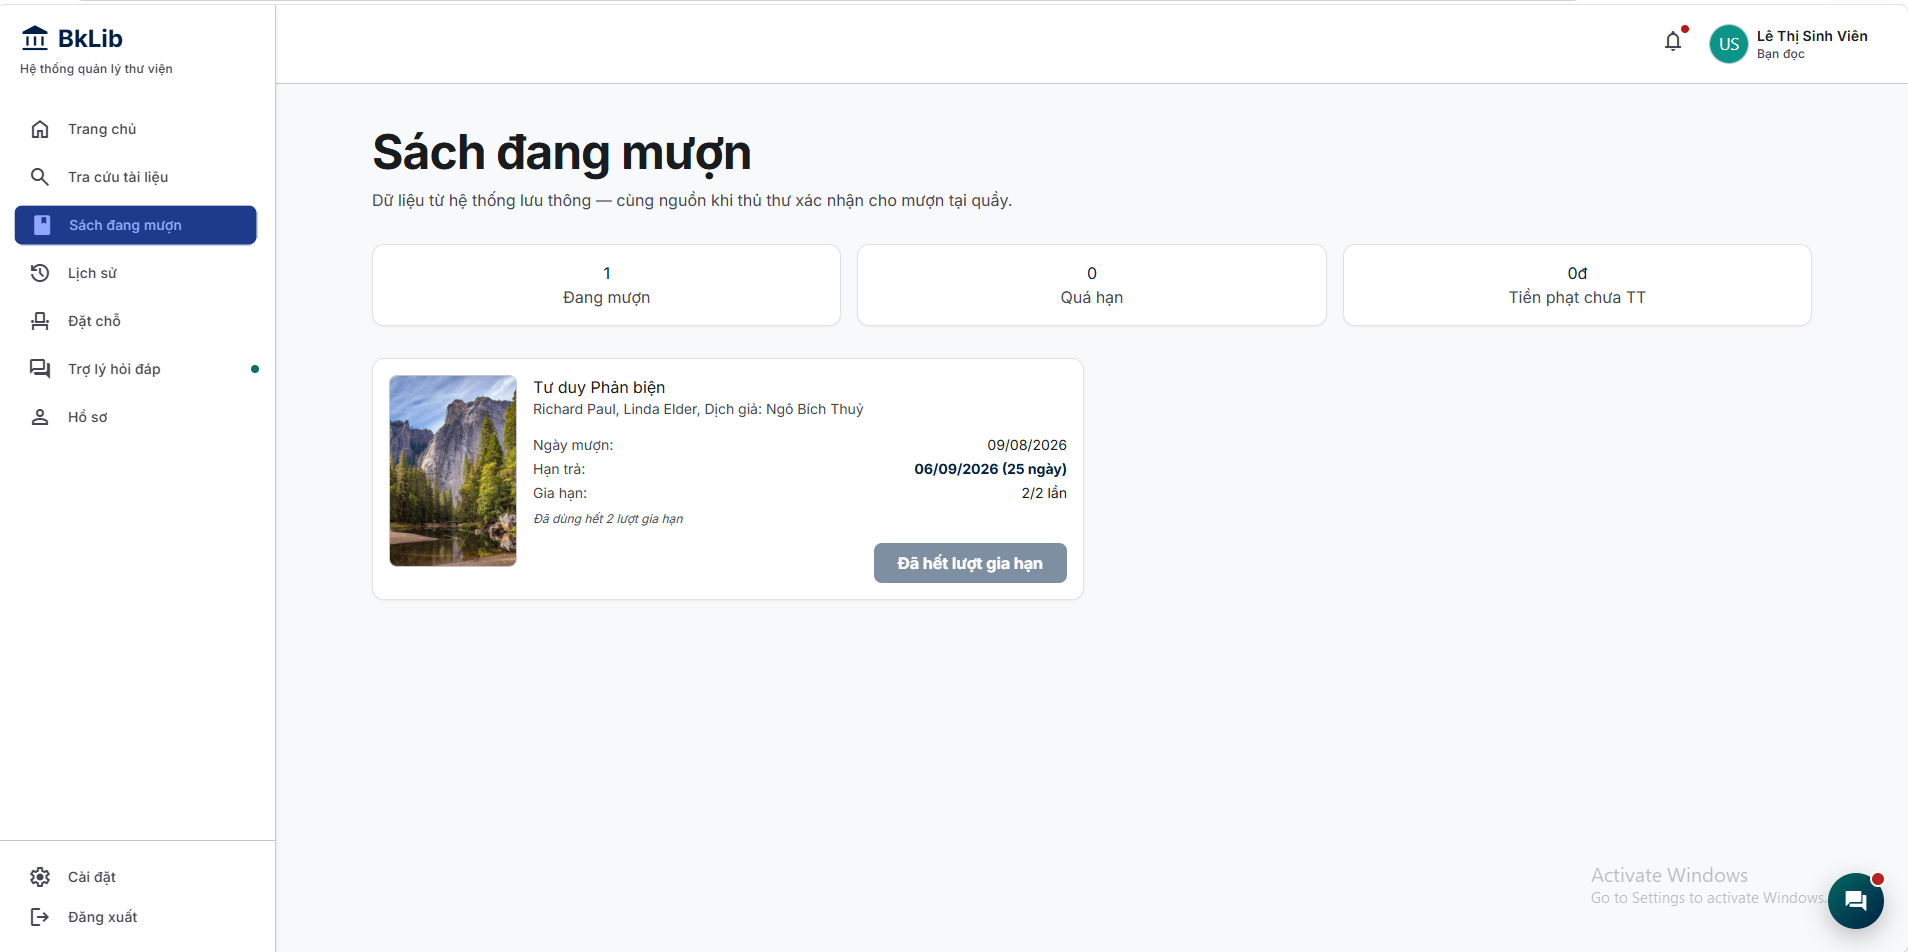
\includegraphics[width=0.95\linewidth]{Images/Reader_SachDangMuon.png}
    \vspace{10pt}
    \caption{Giao diện Quản lý Sách Đang Mượn}
    \label{fig:reader_borrowing}
\end{figure}

\textbf{Bố cục \& Chức năng:} Hiển thị thống kê tổng quan lượt mượn cùng các thẻ tài liệu chi tiết ghi rõ ngày mượn, hạn trả bắt buộc và số lần gia hạn cho phép. Độc giả có thể thực hiện gia hạn trực tiếp, hệ thống sẽ tự động truy vấn các quy tắc lưu thông để tính lại hạn trả hoặc cảnh báo rào cản gia hạn (như có người đặt chỗ hoặc đã đạt giới hạn gia hạn).

\paragraph{Trang Lịch sử Mượn Trả}
Sổ nhật ký lịch sử ghi lại các giao dịch trước đây, các tài liệu đã trả và giao dịch tài chính.

\begin{figure}[H]
    \centering
    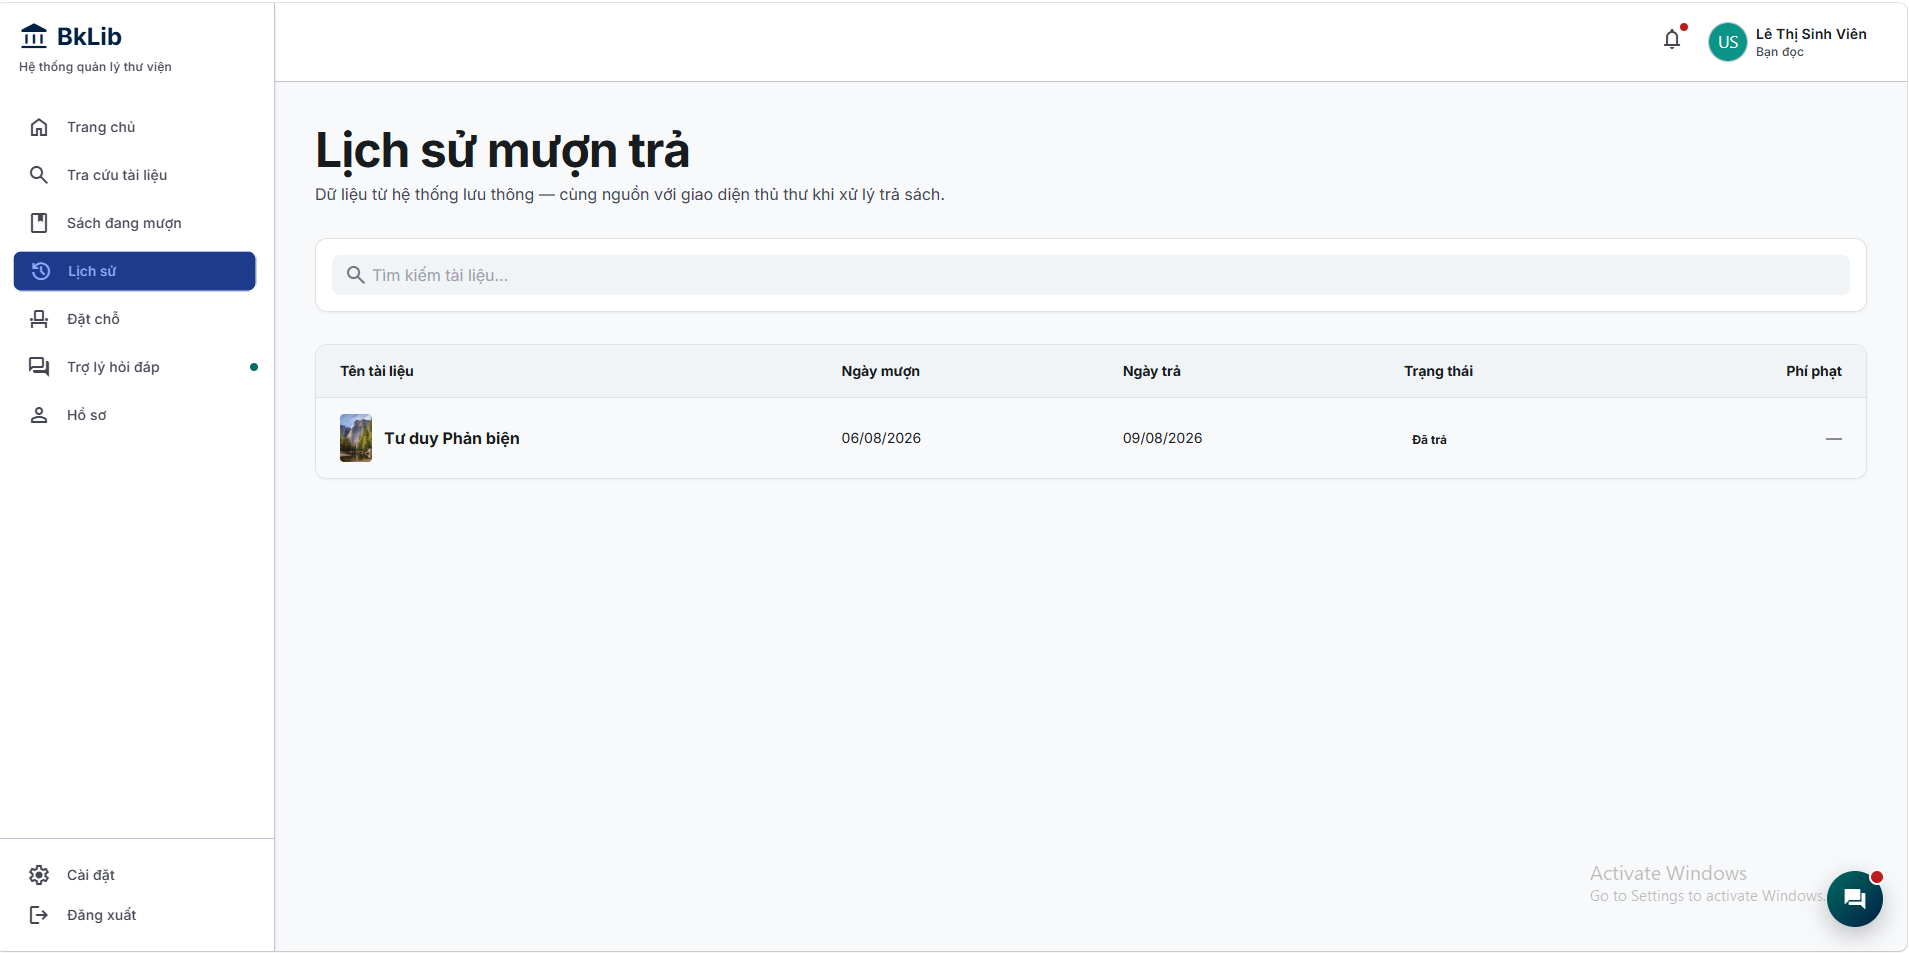
\includegraphics[width=0.95\linewidth]{Images/Reader_LichSu.png}
    \vspace{10pt}
    \caption{Giao diện Lịch sử Mượn Trả}
    \label{fig:reader_history}
\end{figure}

\textbf{Bố cục \& Chức năng:} Bảng cấu trúc chứa tên sách, ngày mượn, mốc thời gian trả thực tế, huy hiệu trạng thái hoàn thành và bản ghi tiền phạt. Hỗ trợ sắp xếp cột phía máy khách và bộ lọc theo khoảng thời gian để độc giả tự kiểm toán tài khoản.

\paragraph{Trang Quản lý Đặt Giữ Chỗ}
Theo dõi vị trí hàng chờ đặt chỗ và thông báo sách đã về cho các tài liệu đang hết hàng.

\begin{figure}[H]
    \centering
    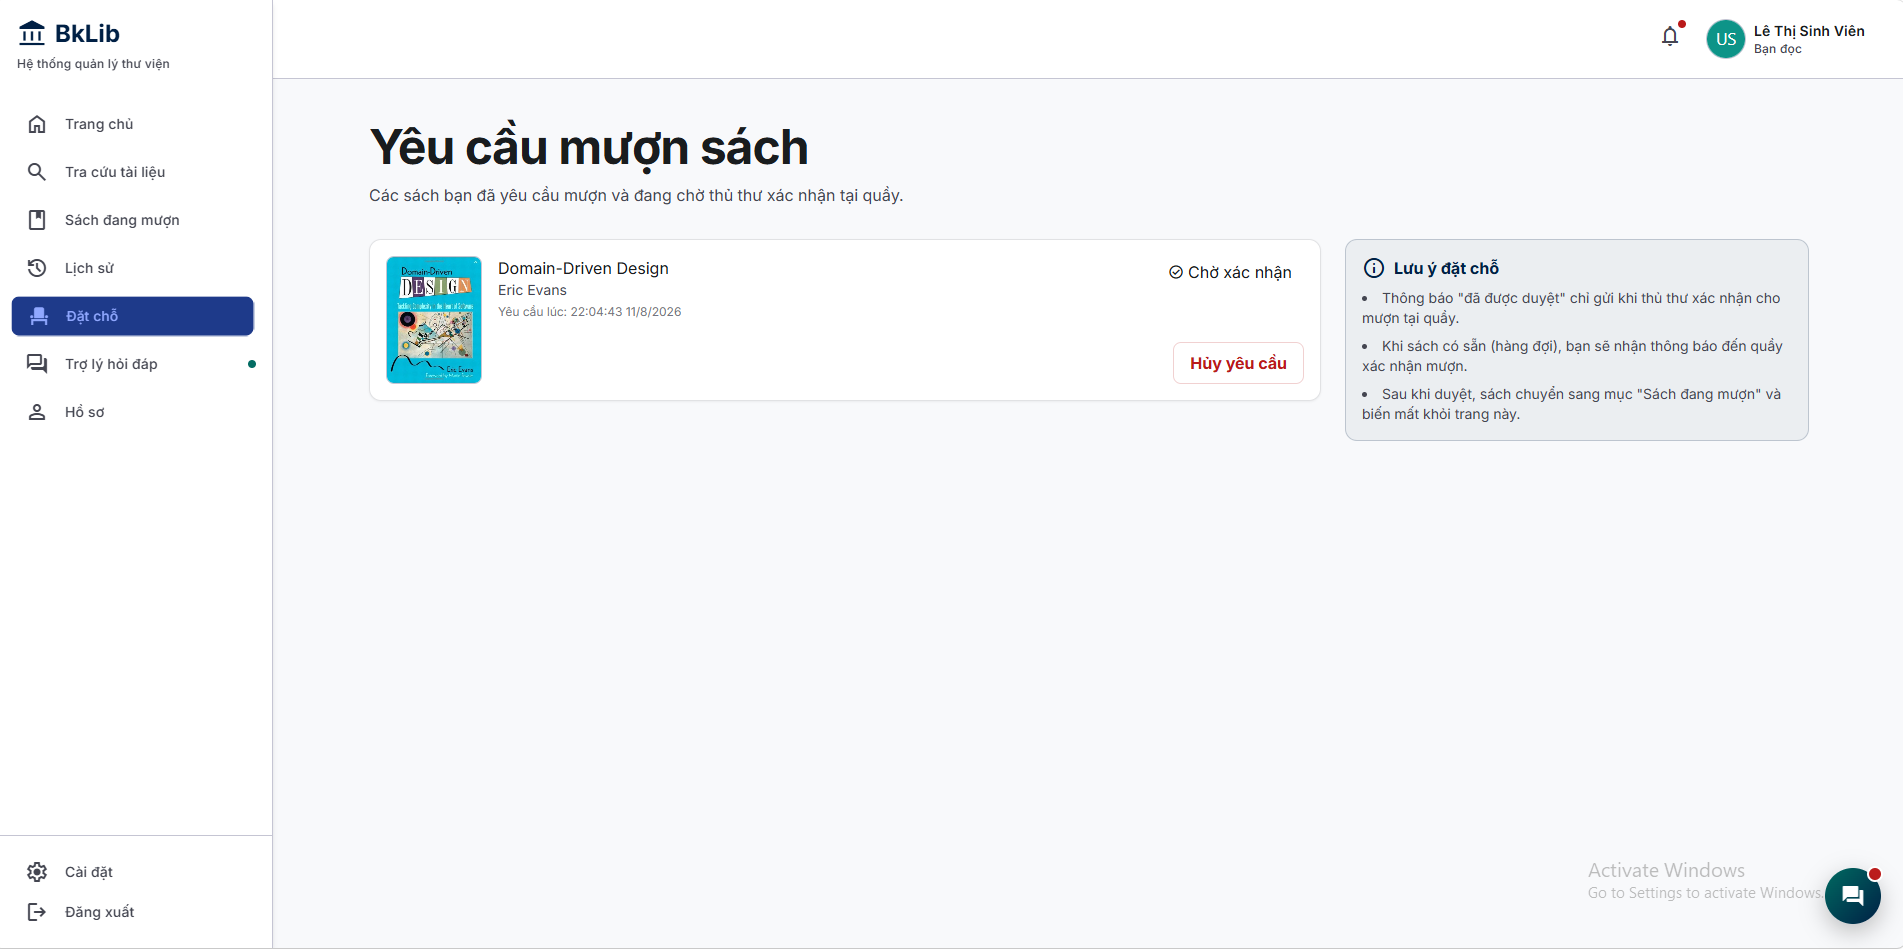
\includegraphics[width=0.95\linewidth]{Images/Reader_DatCho.png}
    \vspace{10pt}
    \caption{Giao diện Quản lý Đặt Giữ Chỗ}
    \label{fig:reader_reservation}
\end{figure}

\textbf{Bố cục \& Chức năng:} Liệt kê các lượt đặt chỗ đang hoạt động với thứ tự hàng chờ, khoảng thời gian chờ nhận sách cho các thông báo sẵn sàng lấy sách, nút hủy đặt chỗ và bảng hướng dẫn chi tiết về quy định đặt chỗ và thời hạn lấy sách của thư viện.

\paragraph{Cửa sổ Trò chuyện Trợ lý Ảo AI}
Widget trợ lý AI tương tác hỗ trợ giao tiếp ngôn ngữ tự nhiên, Q\&A và gợi ý ngữ nghĩa.

\begin{figure}[H]
    \centering
    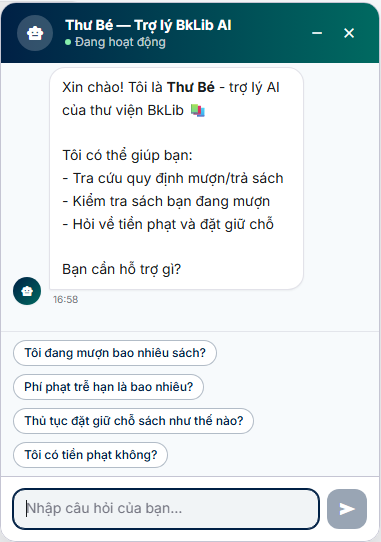
\includegraphics[width=0.45\linewidth]{Images/Reader_ChatbotAI.png}
    \vspace{10pt}
    \caption{Giao diện Cửa sổ Trò chuyện Trợ lý Ảo}
    \label{fig:reader_chatbot}
\end{figure}

\textbf{Bố cục \& Chức năng:} Giao diện trò chuyện nổi sử dụng backend RAG (Retrieval-Augmented Generation) kết hợp. Cung cấp các gợi ý câu hỏi, luồng tin nhắn phản hồi dạng streaming và các liên kết trực tiếp tới trang chi tiết sách được tạo từ các truy vấn tương đồng ngữ nghĩa.

\paragraph{Trang Hồ sơ Cá nhân \& Cài đặt}
Quản lý tài khoản độc giả, thông tin bảo mật và tùy chọn truyền thông.

\begin{figure}[H]
    \centering
    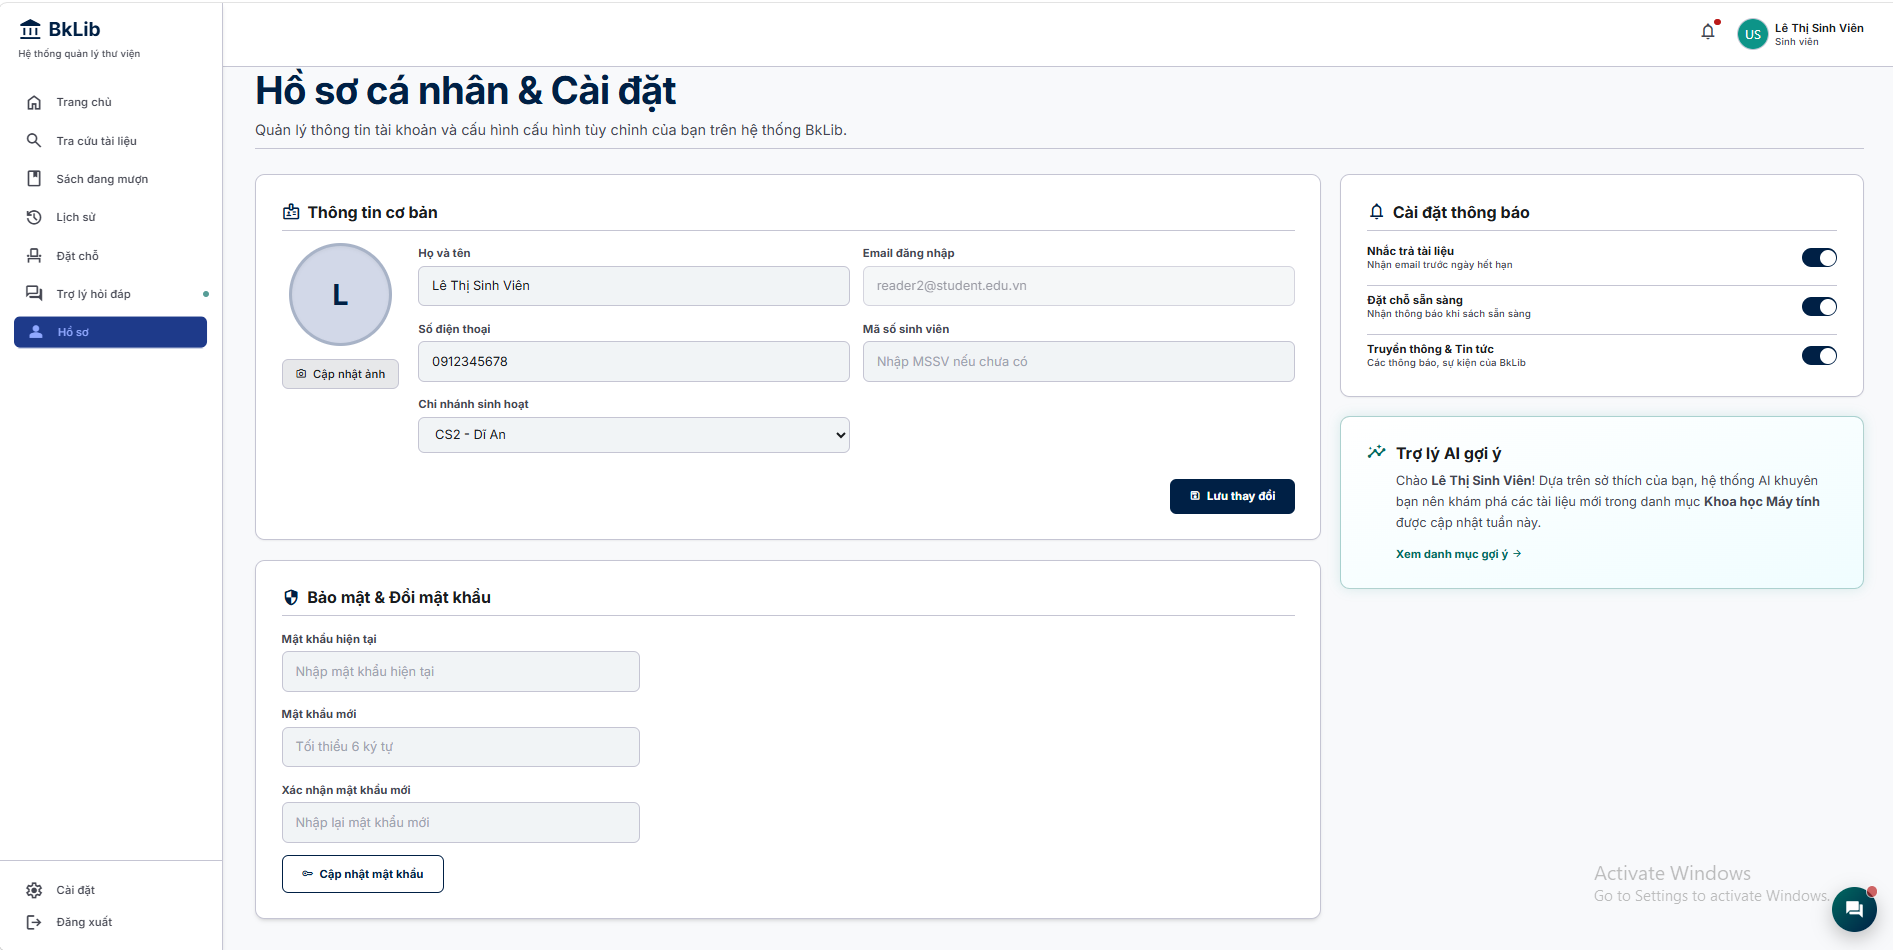
\includegraphics[width=0.95\linewidth]{Images/Reader_HoSoCaiDat.png}
    \vspace{10pt}
    \caption{Giao diện Hồ sơ Cá nhân và Cài đặt}
    \label{fig:reader_profile}
\end{figure}

\textbf{Bố cục \& Chức năng:} Chứa các biểu mẫu chỉnh sửa thông tin liên hệ, công cụ đổi mật khẩu, công tắc chuyển đổi kênh thông báo đa kênh (Email, SMS, In-App) và lưới gợi ý sách cá nhân hóa dựa trên lịch sử đọc của độc giả.

\subsubsection{Các Điểm sáng Hiện thực Kỹ thuật}

Trợ lý Ảo sử dụng các vector nhúng được tạo qua \texttt{SentenceTransformer} và lưu trữ trong bộ sưu tập \texttt{ChromaDB} để truy xuất các đoạn ngữ cảnh phù hợp nhất cho câu hỏi của độc giả.

\begin{lstlisting}[language=Python, caption={Truy xuất Vector ChromaDB cho RAG (ai-service/app/services/rag\_service.py)}, label={lst:rag_retrieval}]
def retrieve_context(query: str, top_k: int = 3) -> str:
    """
    Retrieve top-k relevant text chunks for a query from ChromaDB vector collection.
    Formats results with segment headers to feed into LLM prompt context.
    """
    if _collection is None or _collection.count() == 0:
        return ""

    embedder = get_embeddings()
    query_embedding = embedder.encode([query]).tolist()

    results = _collection.query(
        query_embeddings=query_embedding,
        n_results=min(top_k, _collection.count()),
    )
    docs = results.get("documents", [[]])[0]
    if not docs:
        return ""

    return "\n\n---\n\n".join([f"[Chunk {i+1}]: {doc}" for i, doc in enumerate(docs)])
\end{lstlisting}

% =========================================================================
% SECTION 5.4: LIBRARIAN MODULE
% =========================================================================
\subsection{Mô-đun Thủ thư}

Mô-đun Thủ thư hỗ trợ nhân viên thư viện thực hiện các hoạt động hằng ngày tại quầy, quản lý việc mượn trả tài liệu, duy trì dữ liệu tả danh mục, tính toán phí phạt, gửi thông báo hệ thống và phân tích hiệu suất chi nhánh.

\subsubsection{Hiện thực Giao diện Người dùng}

\paragraph{Trang chủ}
Bảng điều khiển vận hành làm nổi bật các nhiệm vụ hằng ngày, chỉ số trạng thái chi nhánh và hàng chờ xử lý khẩn cấp.

\begin{figure}[H]
    \centering
    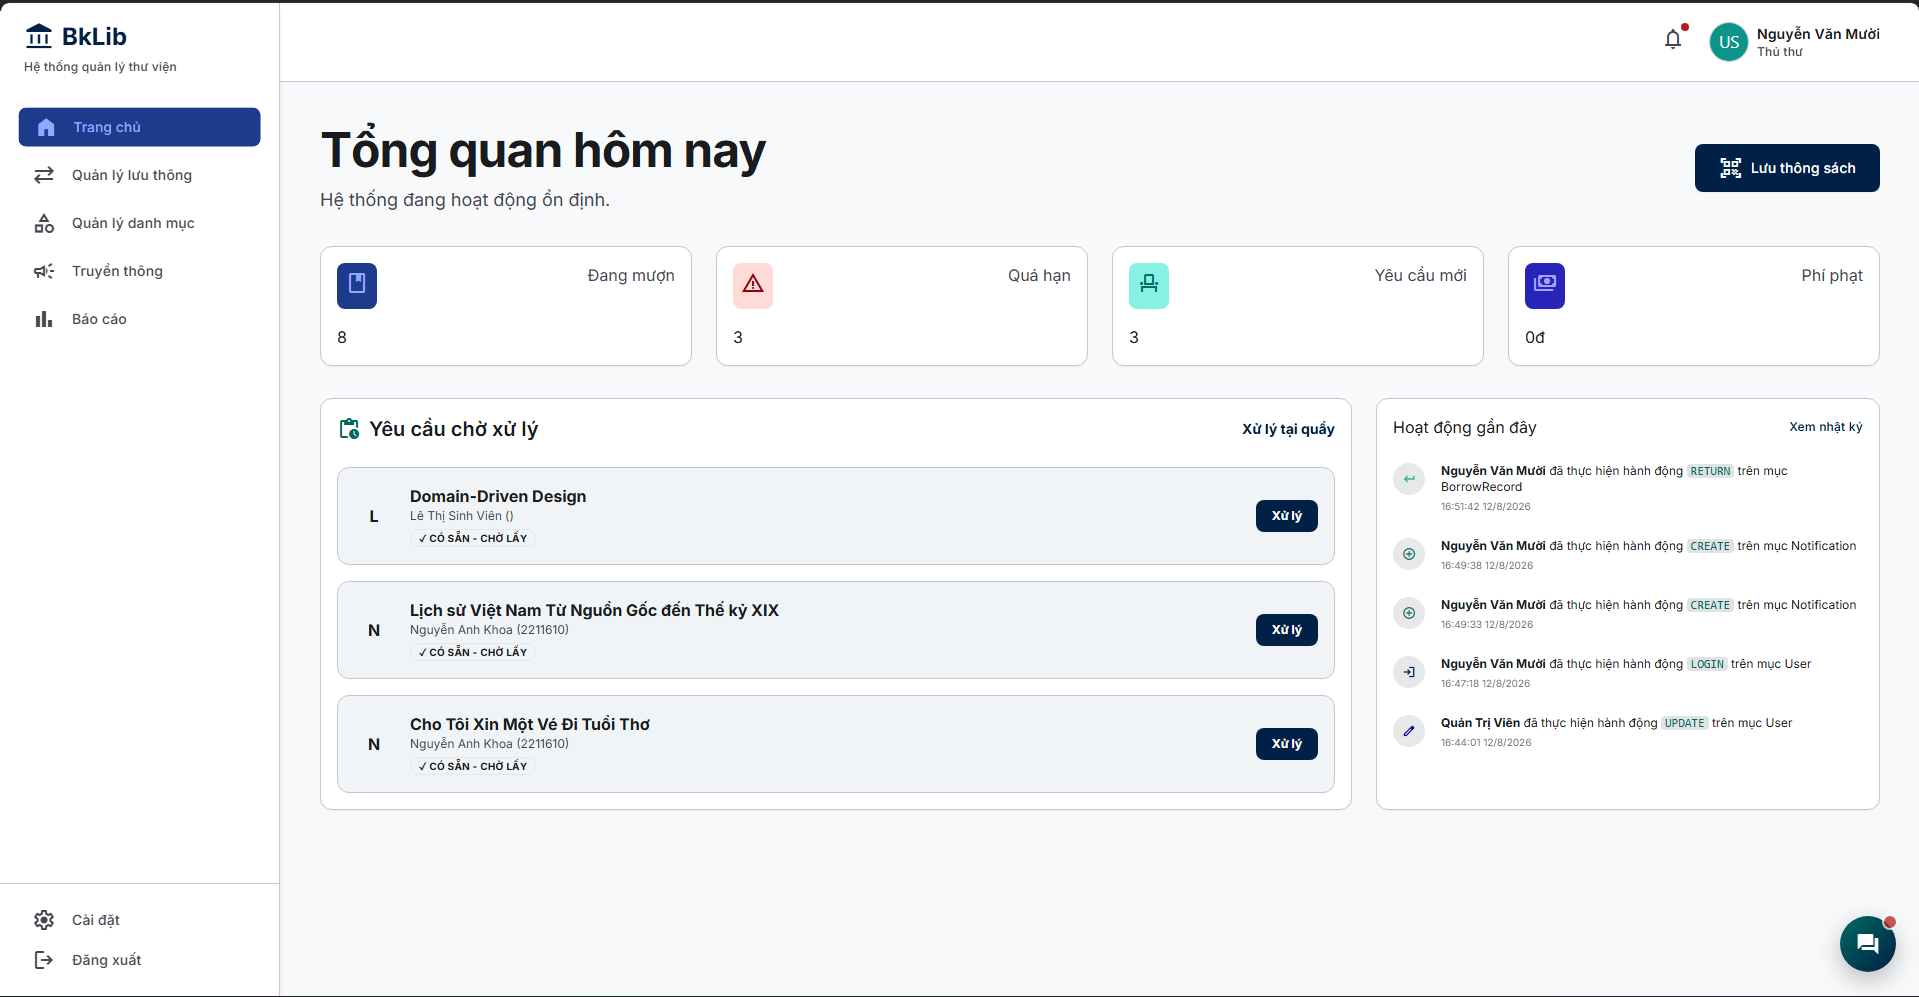
\includegraphics[width=0.95\linewidth]{Images/Librarian_TrangChu.png}
    \vspace{10pt}
    \caption{Giao diện Trang chủ Mô-đun Thủ thư}
    \label{fig:librarian_homepage}
\end{figure}

\textbf{Bố cục \& Chức năng:} Cung cấp các lối tắt truy cập nhanh (Lưu thông, Biên mục, Thông báo, Báo cáo), chỉ số hiệu suất quầy theo thời gian thực, hàng chờ đặt chỗ đang chờ xử lý và luồng nhật ký ghi lại các hoạt động mượn trả mới nhất.

\paragraph{Trang Quản lý Lưu thông}
Giao diện xử lý tại quầy được tối ưu hóa cho tốc độ mượn, trả và thanh toán tiền phạt cao.

\begin{figure}[H]
    \centering
    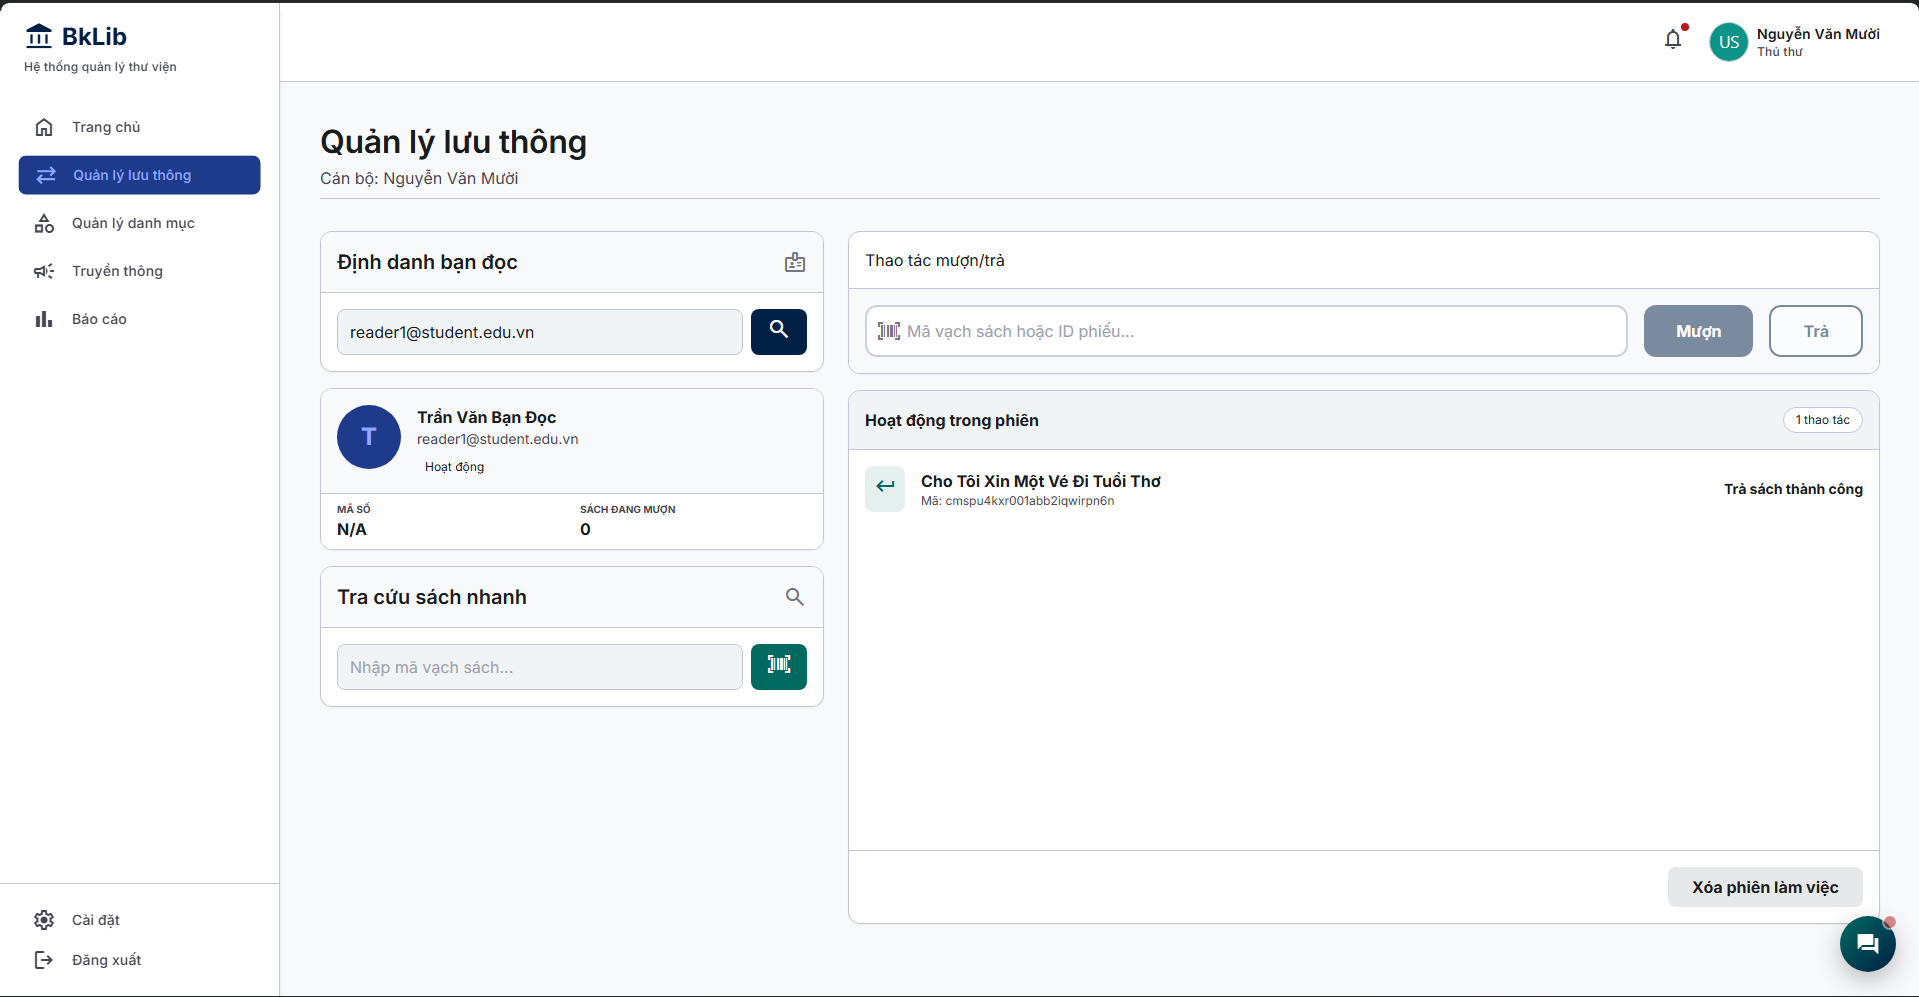
\includegraphics[width=0.95\linewidth]{Images/Librarian_QuanLyLuuThong.png}
    \vspace{10pt}
    \caption{Giao diện Quản lý Lưu thông}
    \label{fig:librarian_circulation}
\end{figure}

\textbf{Bố cục \& Chức năng:} Giao diện hai khung: khung tra cứu Thẻ/ID Độc giả bên trái, và ô quét mã vạch nhanh với tóm tắt giao dịch và xác minh trả sách bên phải. Ngay lập tức xác minh trạng thái tài khoản độc giả, các khoản giữ chỗ quá hạn và tự động tính tiền phạt khi quét mã.

\paragraph{Trang Quản lý Danh mục}
Không gian làm việc quản trị cho dữ liệu tả sách, theo dõi tồn kho và dán mã vạch bản sao vật lý.

\begin{figure}[H]
    \centering
    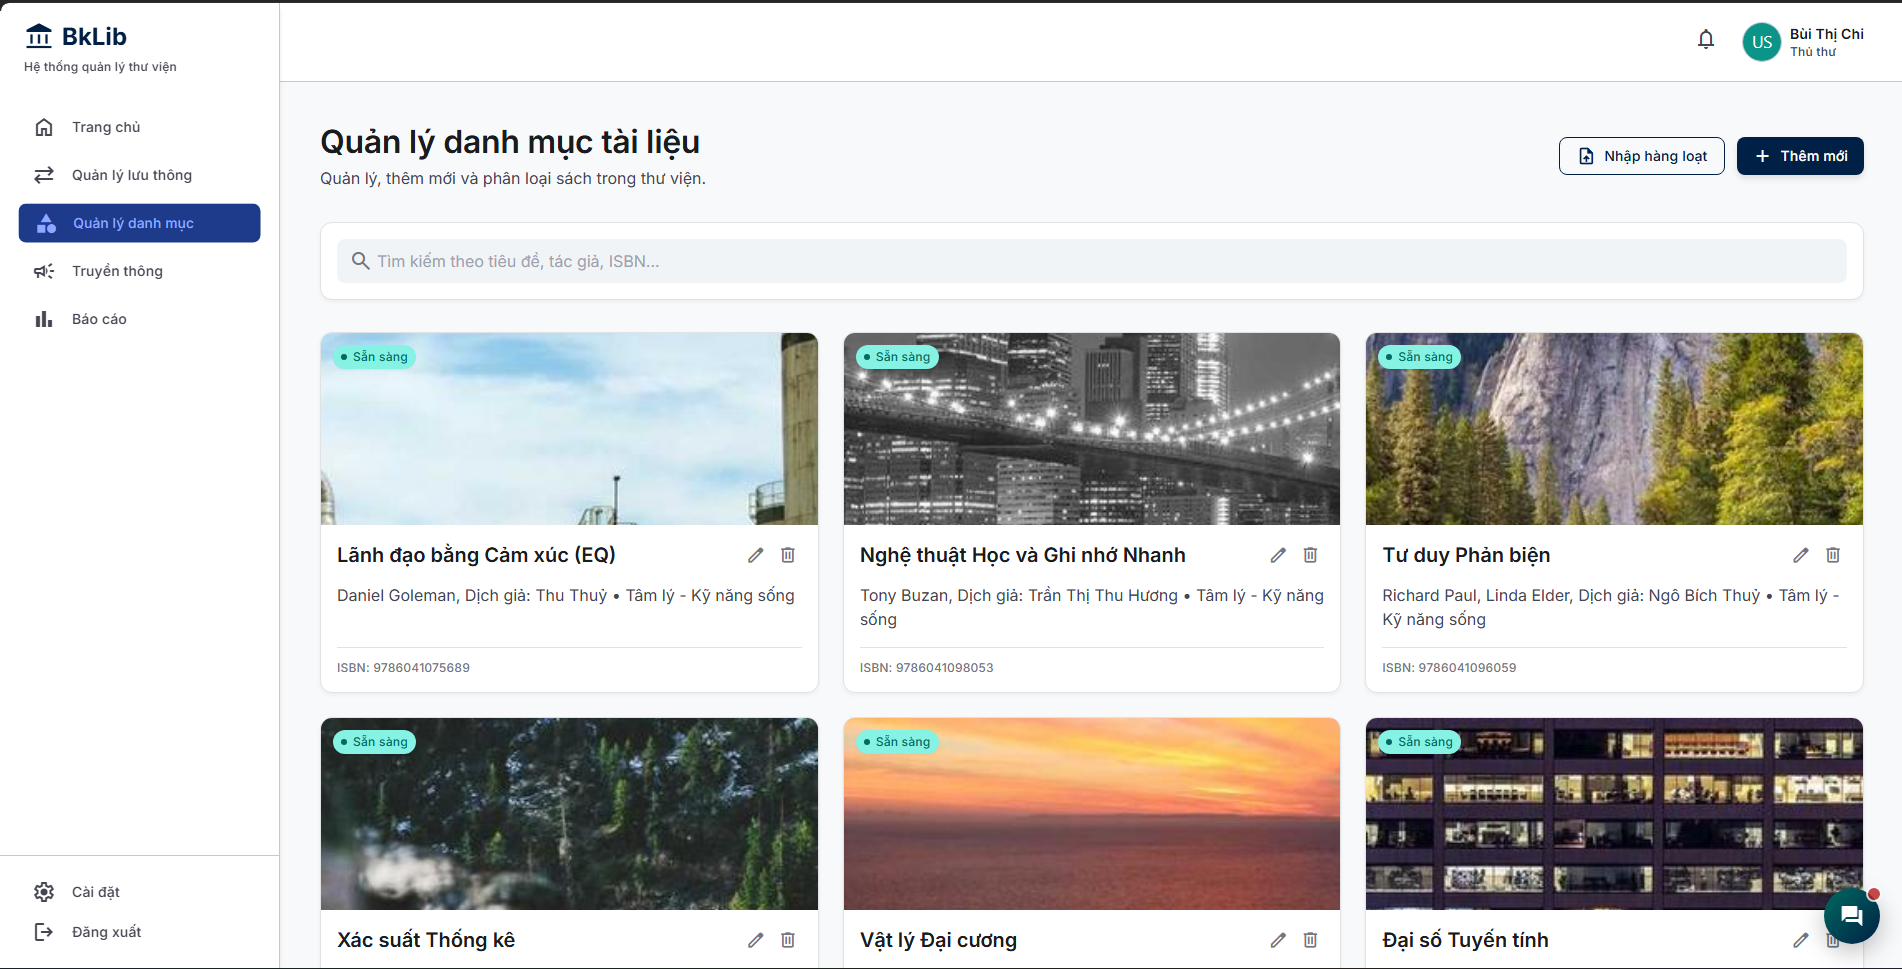
\includegraphics[width=0.95\linewidth]{Images/Librarian_QuanLyDanhMuc.png}
    \vspace{10pt}
    \caption{Giao diện Quản lý Danh mục}
    \label{fig:librarian_catalog}
\end{figure}

\textbf{Bố cục \& Chức năng:} Thanh công cụ tìm kiếm tích hợp tự động lấy dữ liệu qua ISBN, công cụ nhập dữ liệu hàng loạt từ CSV/Excel, biểu mẫu tạo tài liệu modal và bảng tồn kho phân trang hỗ trợ sửa trực tiếp, chuyển đổi trạng thái và tạo mã vạch bản sao.

\paragraph{Trang Quản lý Truyền thông}
Cổng phát thông báo cho các tin tức thư viện và chiến dịch thông báo tới nhóm độc giả mục tiêu.

\begin{figure}[H]
    \centering
    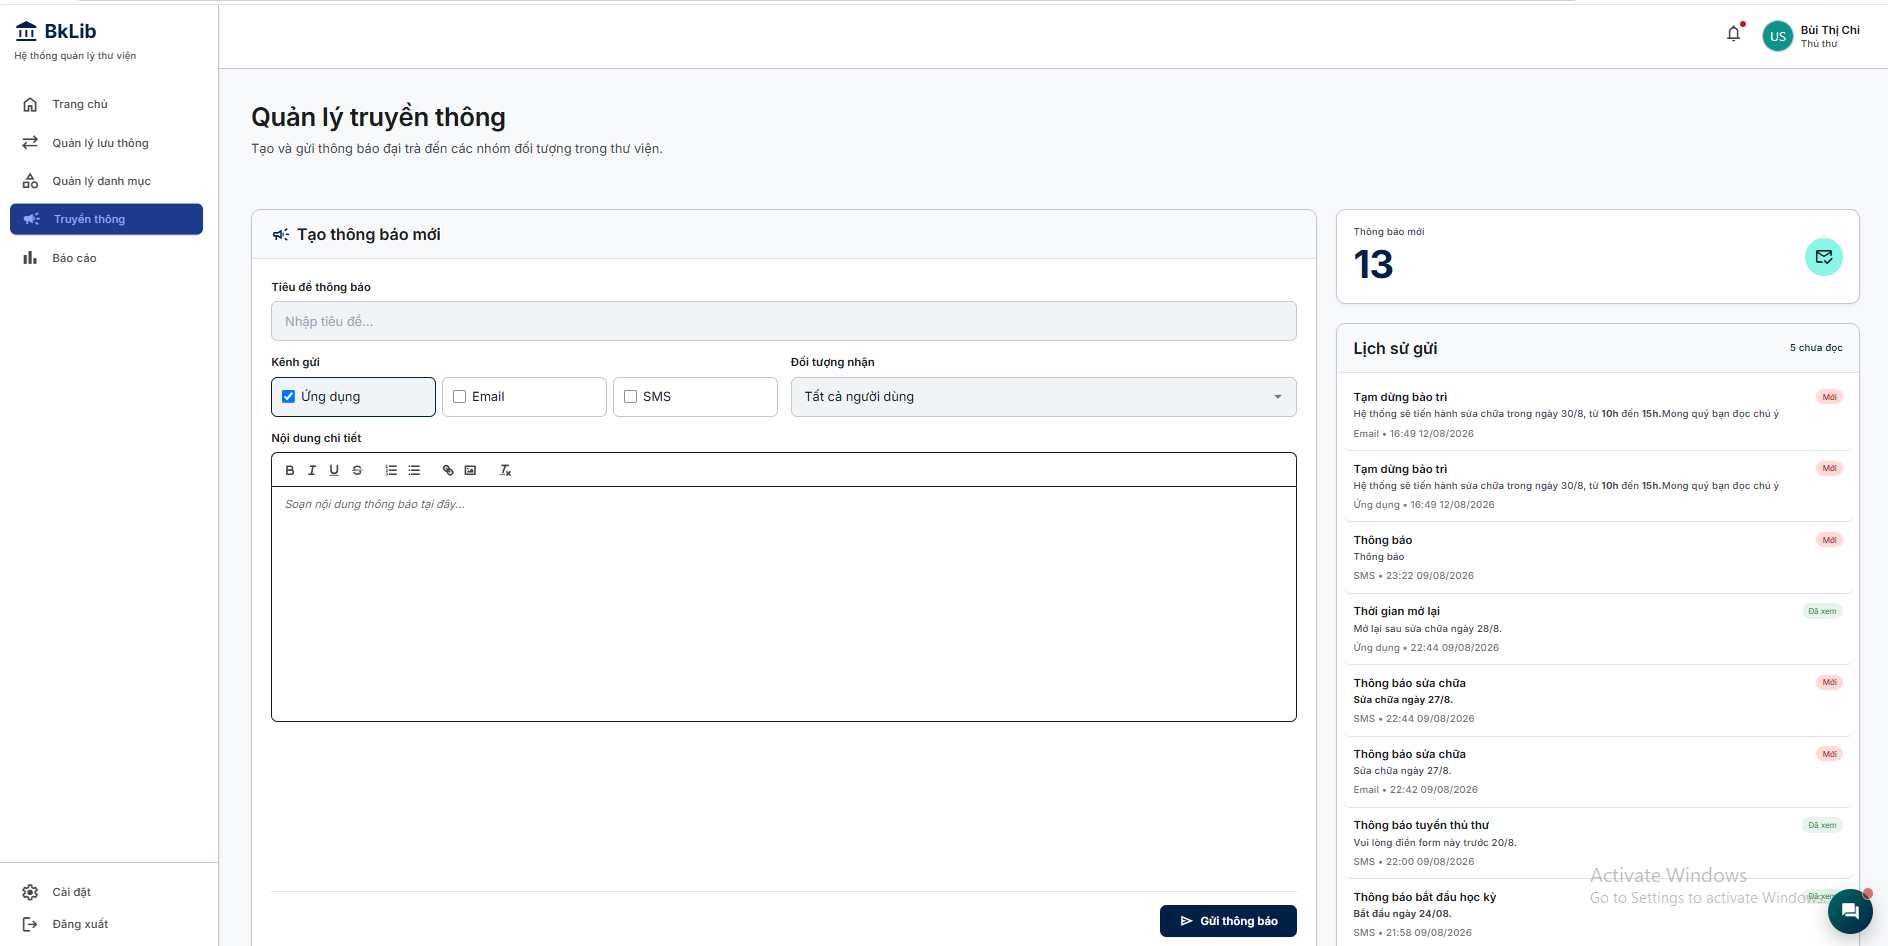
\includegraphics[width=0.95\linewidth]{Images/Librarian_TruyenThong.png}
    \vspace{10pt}
    \caption{Giao diện Quản lý Truyền thông}
    \label{fig:librarian_notification}
\end{figure}

\textbf{Bố cục \& Chức năng:} Trình soạn thảo thông báo văn bản giàu định dạng với tùy chọn chọn đối tượng đích (Tất cả độc giả, Độc giả quá hạn, Nhóm thành viên cụ thể), lựa chọn kênh (In-App, Email) và nhật ký lịch sử gửi ghi rõ tỷ lệ thành công.

\paragraph{Trang Báo cáo \& Phân tích}
Bảng điều khiển trực quan hóa dữ liệu theo dõi lưu lượng lưu thông, mức độ sử dụng bộ sưu tập và chỉ số tài chính.

\begin{figure}[H]
    \centering
    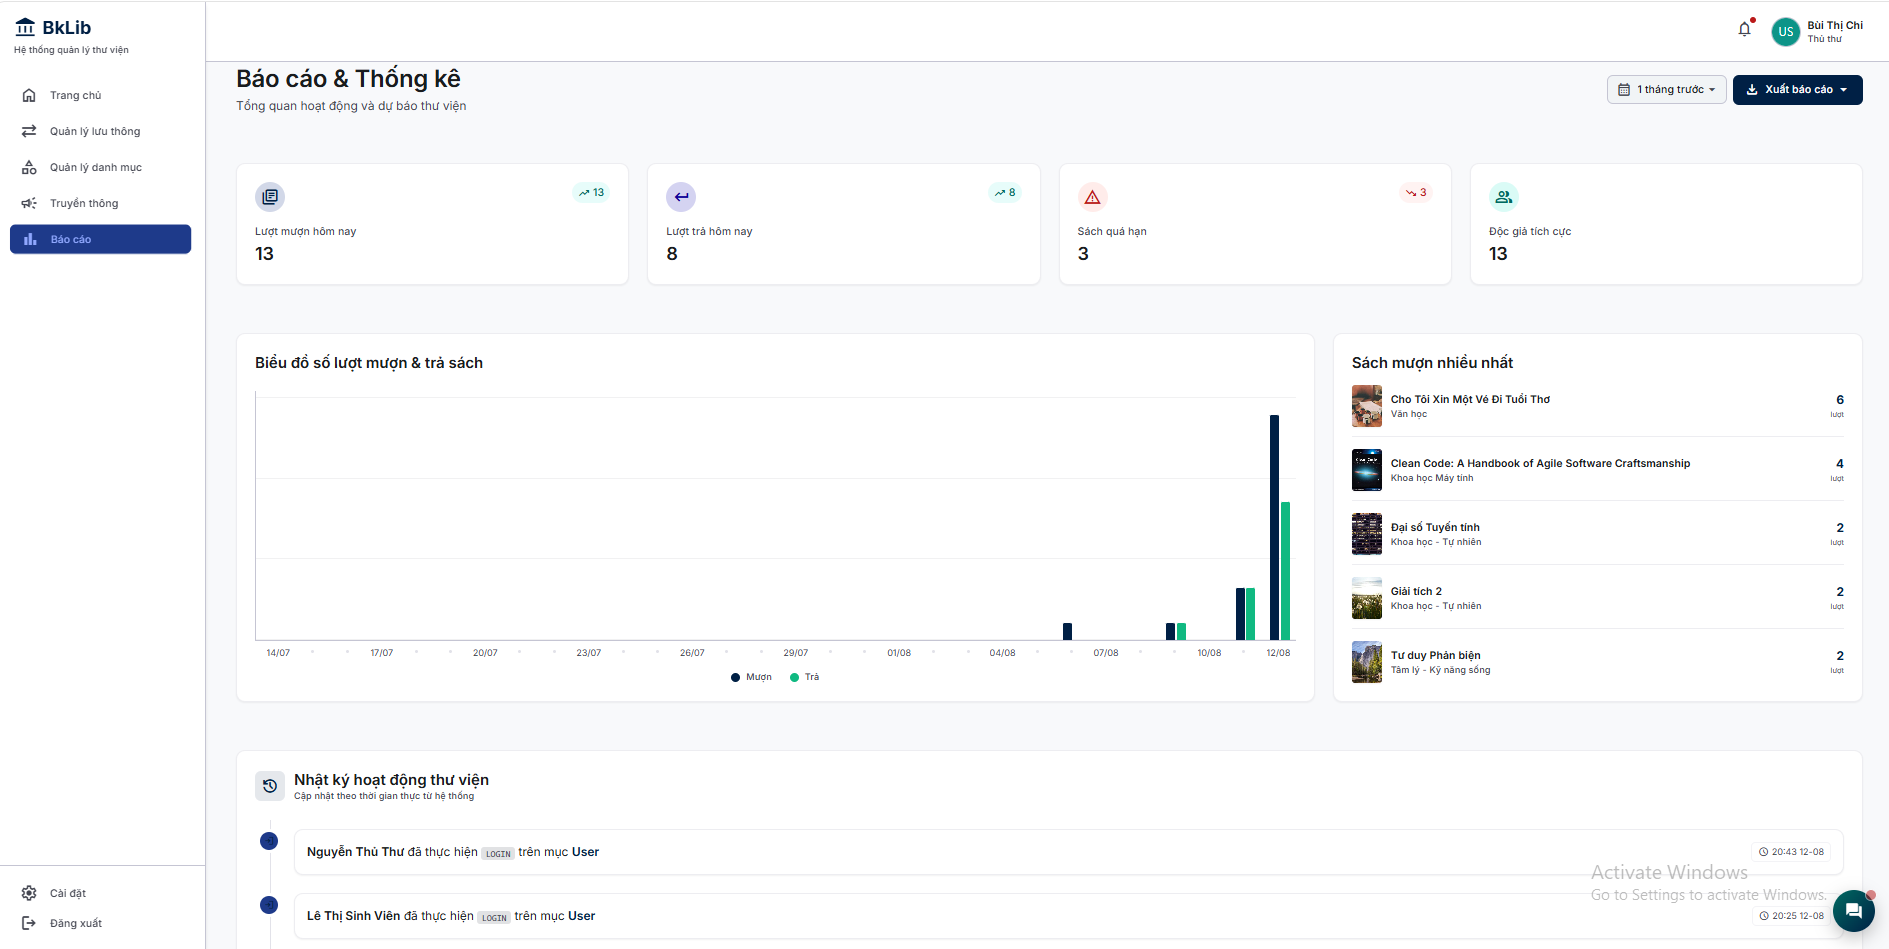
\includegraphics[width=0.95\linewidth]{Images/Librarian_BaoCao.png}
    \vspace{10pt}
    \caption{Giao diện Báo cáo và Phân tích cho Thủ thư}
    \label{fig:librarian_report}
\end{figure}

\textbf{Bố cục \& Chức năng:} Bộ điều khiển khoảng thời gian tương tác, nút xuất dữ liệu (PDF, Excel, CSV), biểu đồ xu hướng lưu thông, xếp hạng sách mượn nhiều nhất và phân tích thu tiền phạt để hỗ trợ kế hoạch bổ sung tài nguyên.

\paragraph{Trang Hồ sơ Cá nhân \& Cài đặt}
Không gian làm việc quản lý tài khoản nhân viên để cập nhật thuộc tính hồ sơ, mật khẩu bảo mật và tùy chọn nhận thông báo.

\begin{figure}[H]
    \centering
    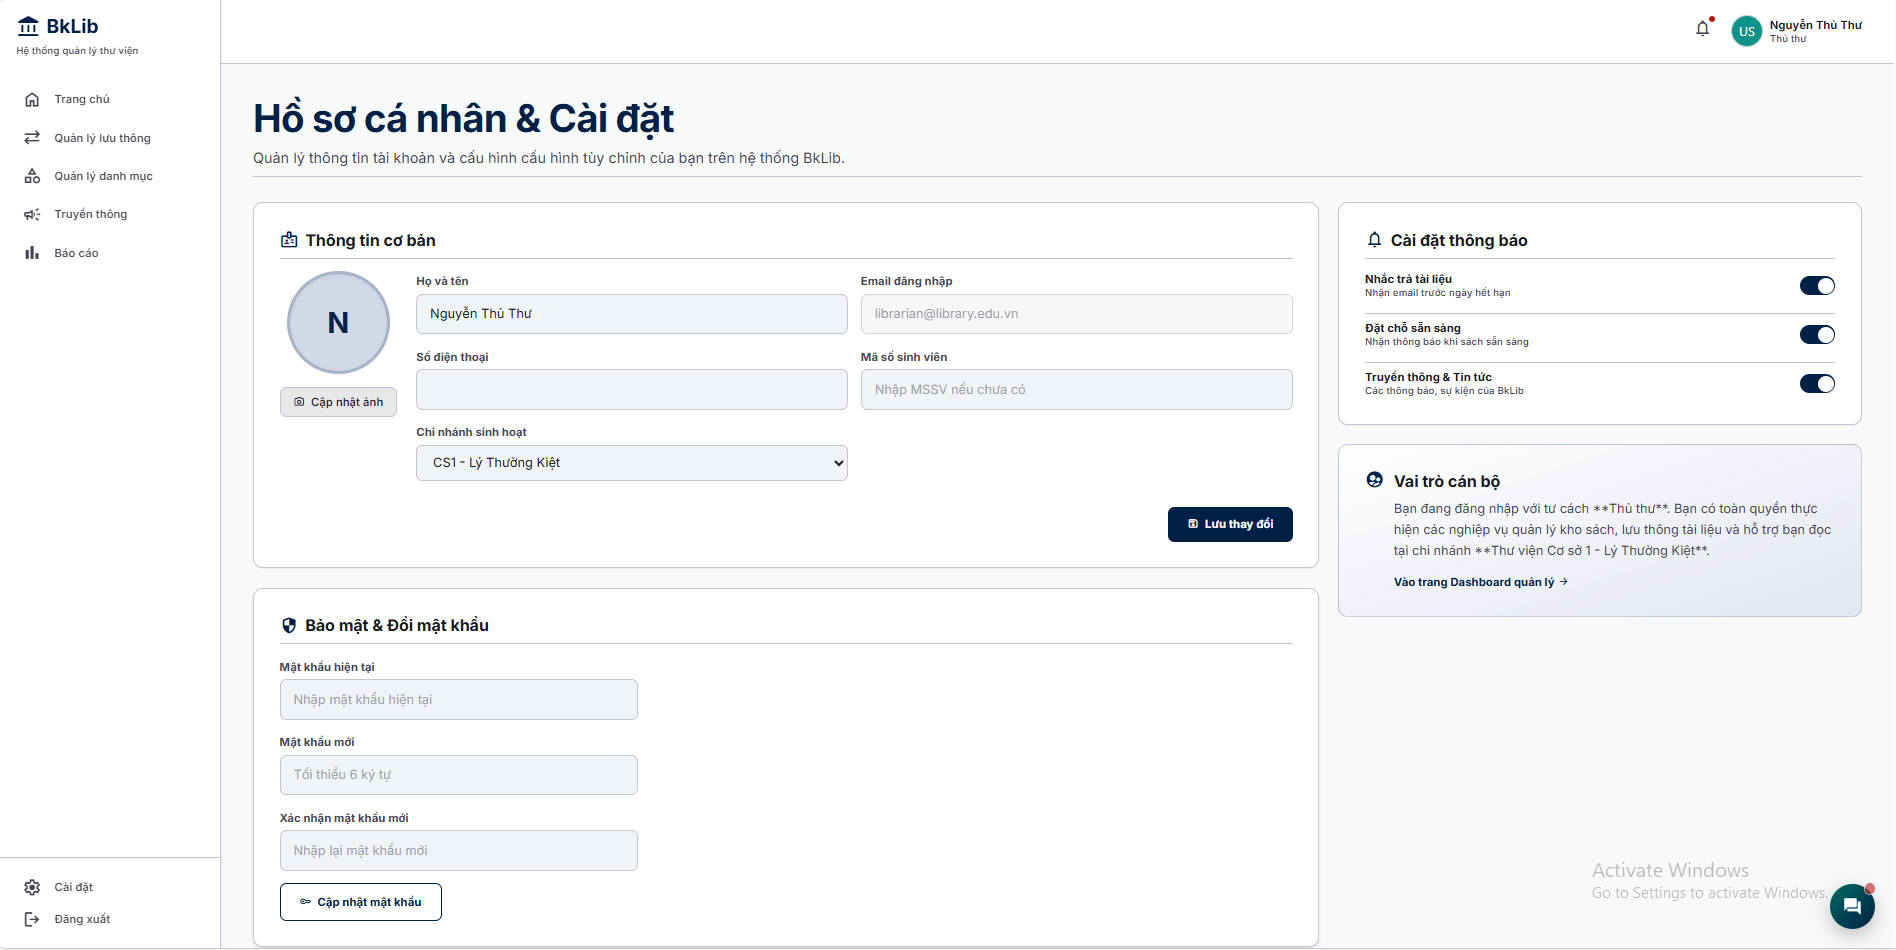
\includegraphics[width=0.95\linewidth]{Images/Librarian_HoSoCaiDat.png}
    \vspace{10pt}
    \caption{Giao diện Hồ sơ Cá nhân và Cài đặt Thủ thư}
    \label{fig:librarian_profile}
\end{figure}

\textbf{Bố cục \& Chức năng:} Được tổ chức thành bố cục bảng điều khiển nhiều thẻ:
\begin{itemize}
    \item \textbf{Khung Thông tin Cơ bản ("Thông tin cơ bản"):} Các trường hồ sơ có thể chỉnh sửa bao gồm họ tên, email đăng nhập, số điện thoại liên hệ, mã cán bộ, bộ chọn chi nhánh làm việc (ví dụ: CS1 - Lý Thường Kiệt) và công cụ cập nhật ảnh đại diện.
    \item \textbf{Bảo mật \& Đổi Mật khẩu ("Bảo mật \& Đổi mật khẩu"):} Công cụ quản lý mật khẩu yêu cầu xác nhận mật khẩu hiện tại trước khi nhập mật khẩu mới.
    \item \textbf{Tùy chọn Thông báo ("Cài đặt thông báo"):} Các công tắc bật/tắt cho các cảnh báo tự động, bao gồm nhắc nhở trả sách, thông báo đặt chỗ đã về và thông báo toàn hệ thống.
    \item \textbf{Tóm tắt Vai trò Cán bộ ("Vai trò cán bộ"):} Thẻ hiển thị các quyền hạn hiện tại, chi nhánh làm việc được phân công và liên kết trực tiếp tới bảng điều khiển quản trị.
\end{itemize}

\subsubsection{Các Điểm sáng Hiện thực Kỹ thuật}

Logic lưu thông tính toán động số ngày quá hạn bằng cách lặp qua các khoảng thời gian mượn trả đồng thời loại trừ các ngày nghỉ lễ chính thức của thư viện được cấu hình trong cài đặt hệ thống.

\begin{lstlisting}[caption={Tính số Ngày Quá hạn có Nhận biết Ngày Lễ (backend-express/src/modules/circulation/circulation.service.ts)}, label={lst:calc_overdue}]
const calcOverdueDays = async (dueDate: Date, returnDate: Date): Promise<number> => {
  if (returnDate <= dueDate) return 0;

  // Retrieve holiday array from system configuration
  const holidayConfig = await getConfig(CONFIG_KEYS.HOLIDAY_DATES, '[]');
  const holidays: string[] = JSON.parse(holidayConfig);

  let overdueDays = 0;
  const cursor = new Date(dueDate);
  cursor.setDate(cursor.getDate() + 1);

  // Iterate day-by-day excluding scheduled holidays
  while (cursor <= returnDate) {
    const dateStr = cursor.toISOString().split('T')[0];
    if (!holidays.includes(dateStr)) {
      overdueDays++;
    }
    cursor.setDate(cursor.getDate() + 1);
  }
  return overdueDays;
};
\end{lstlisting}

% =========================================================================
% SECTION 5.5: ADMINISTRATOR MODULE
% =========================================================================
\subsection{Mô-đun Quản trị viên}

Mô-đun Quản trị viên cung cấp khả năng quản trị cấp cao nhất cho nền tảng. Cho phép quản trị viên quản lý Kiểm soát Truy cập Dựa trên Vai trò (RBAC), cấu hình thiết lập hệ thống, quản lý mạng lưới chi nhánh, kiểm toán nhật ký hệ thống, giám sát sức khỏe hạ tầng và thực hiện các thao tác sao lưu, khôi phục cơ sở dữ liệu khi có sự cố.

\subsubsection{Hiện thực Giao diện Người dùng}

\paragraph{Bảng điều khiển Tổng quan Hệ thống}
Bảng điều khiển giám sát hạ tầng, tải máy chủ và thống kê sử dụng cấp cao.

\begin{figure}[H]
    \centering
    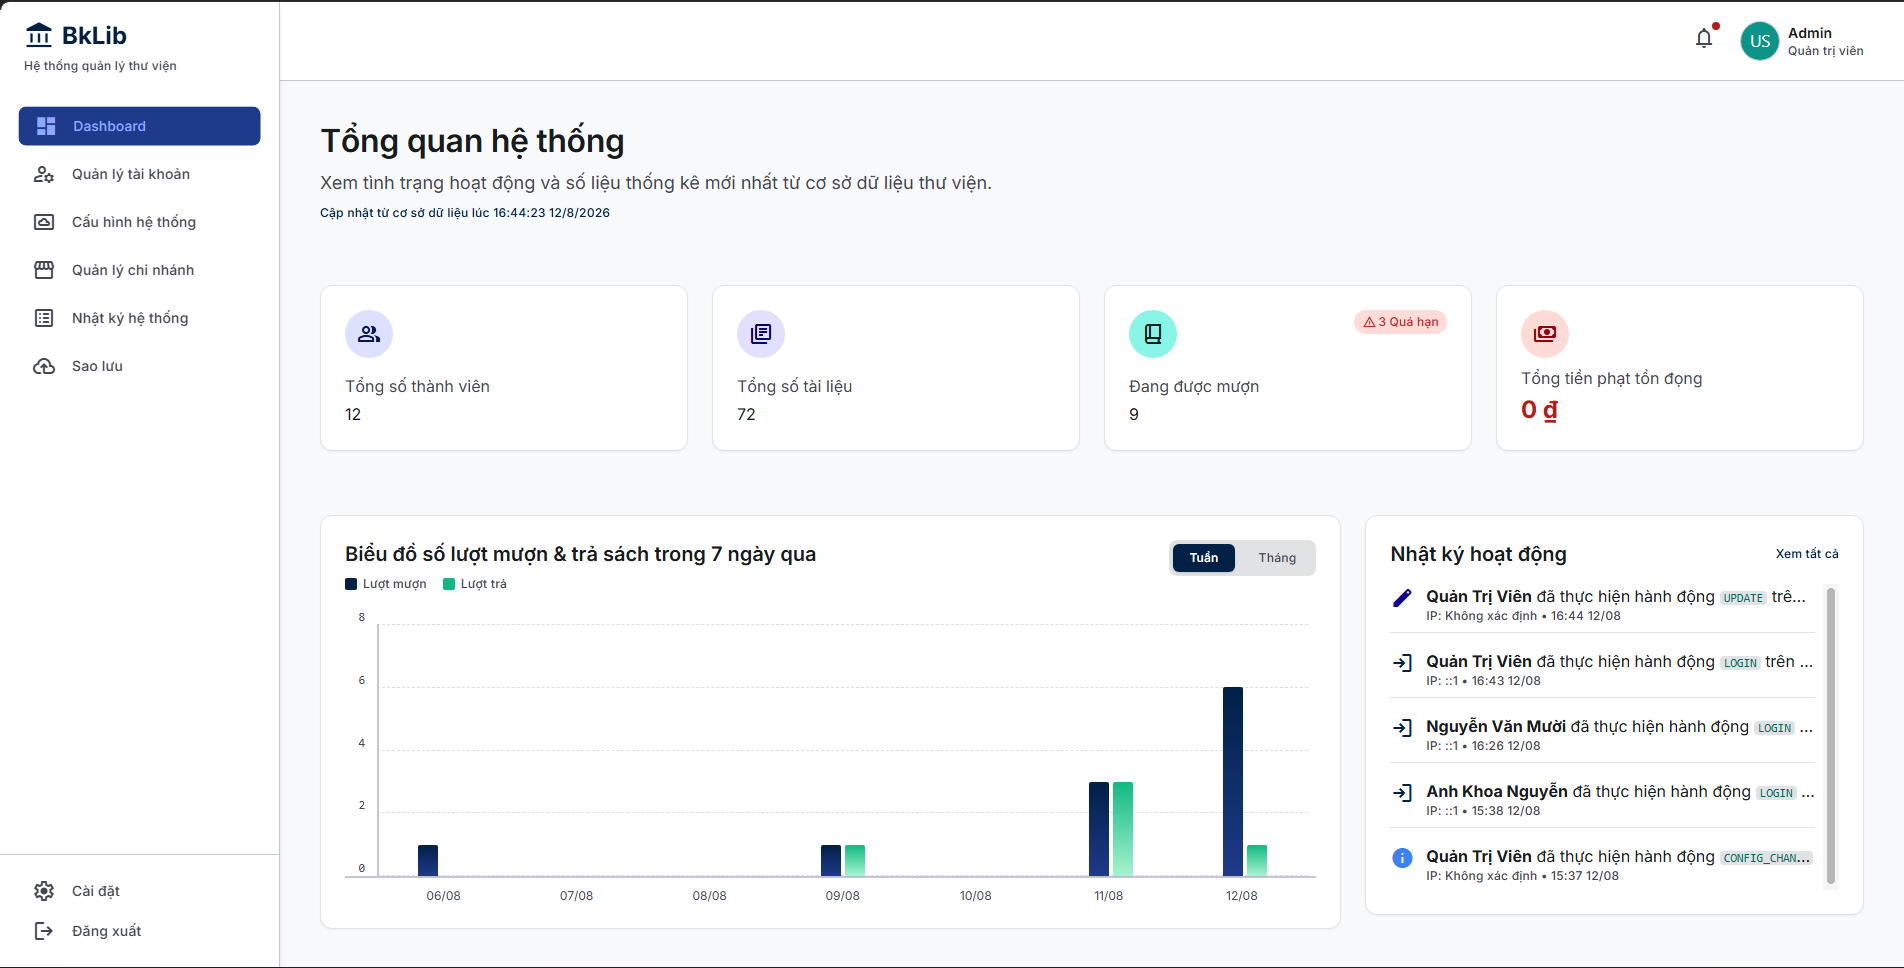
\includegraphics[width=0.95\linewidth]{Images/Admin_Dashboard.png}
    \vspace{10pt}
    \caption{Bảng điều khiển Tổng quan Hệ thống cho Quản trị viên}
    \label{fig:admin_dashboard}
\end{figure}

\textbf{Bố cục \& Chức năng:} Hiển thị các thẻ chỉ số hệ thống (Tổng số tài khoản đang hoạt động, Quy mô danh mục, Số phiên làm việc), chỉ báo lưu trữ cơ sở dữ liệu đám mây, đồ thị lưu lượng API và các cảnh báo an ninh theo thời gian thực.

\paragraph{Trang Quản lý Tài khoản Người dùng}
Không gian làm việc tập trung cho vòng đời tài khoản người dùng, phân quyền và quản lý vai trò.

\begin{figure}[H]
    \centering
    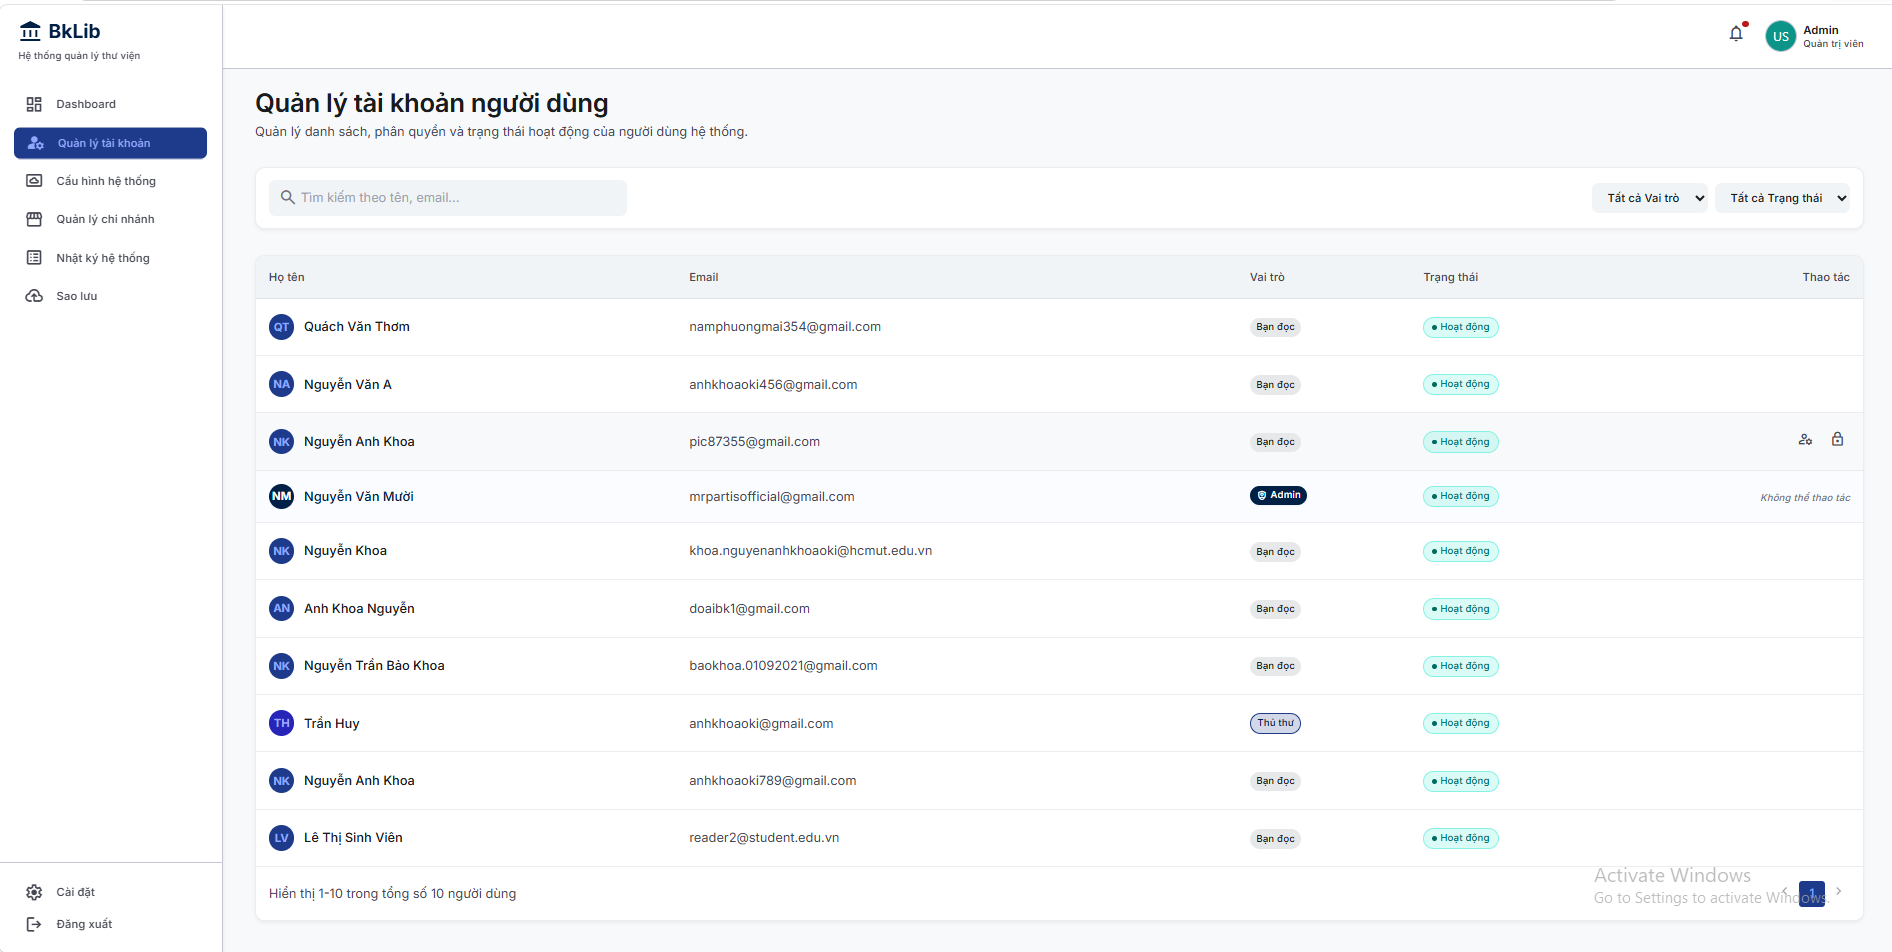
\includegraphics[width=0.95\linewidth]{Images/Admin_QuanLyTaiKhoan.png}
    \vspace{10pt}
    \caption{Giao diện Quản lý Tài khoản Người dùng}
    \label{fig:admin_user_management}
\end{figure}

\textbf{Bố cục \& Chức năng:} Danh mục người dùng phân trang với bộ lọc vai trò (Độc giả, Thủ thư, Admin), nút mở modal tạo tài khoản, công cụ gán quyền RBAC và công tắc khóa/mở khóa tài khoản khẩn cấp.

\paragraph{Trang Cấu hình Hệ thống}
Giao diện quản trị tập trung để định nghĩa các tham số vận hành hệ thống, quy tắc lưu thông và cấu trúc phạt.

\begin{figure}[H]
    \centering
    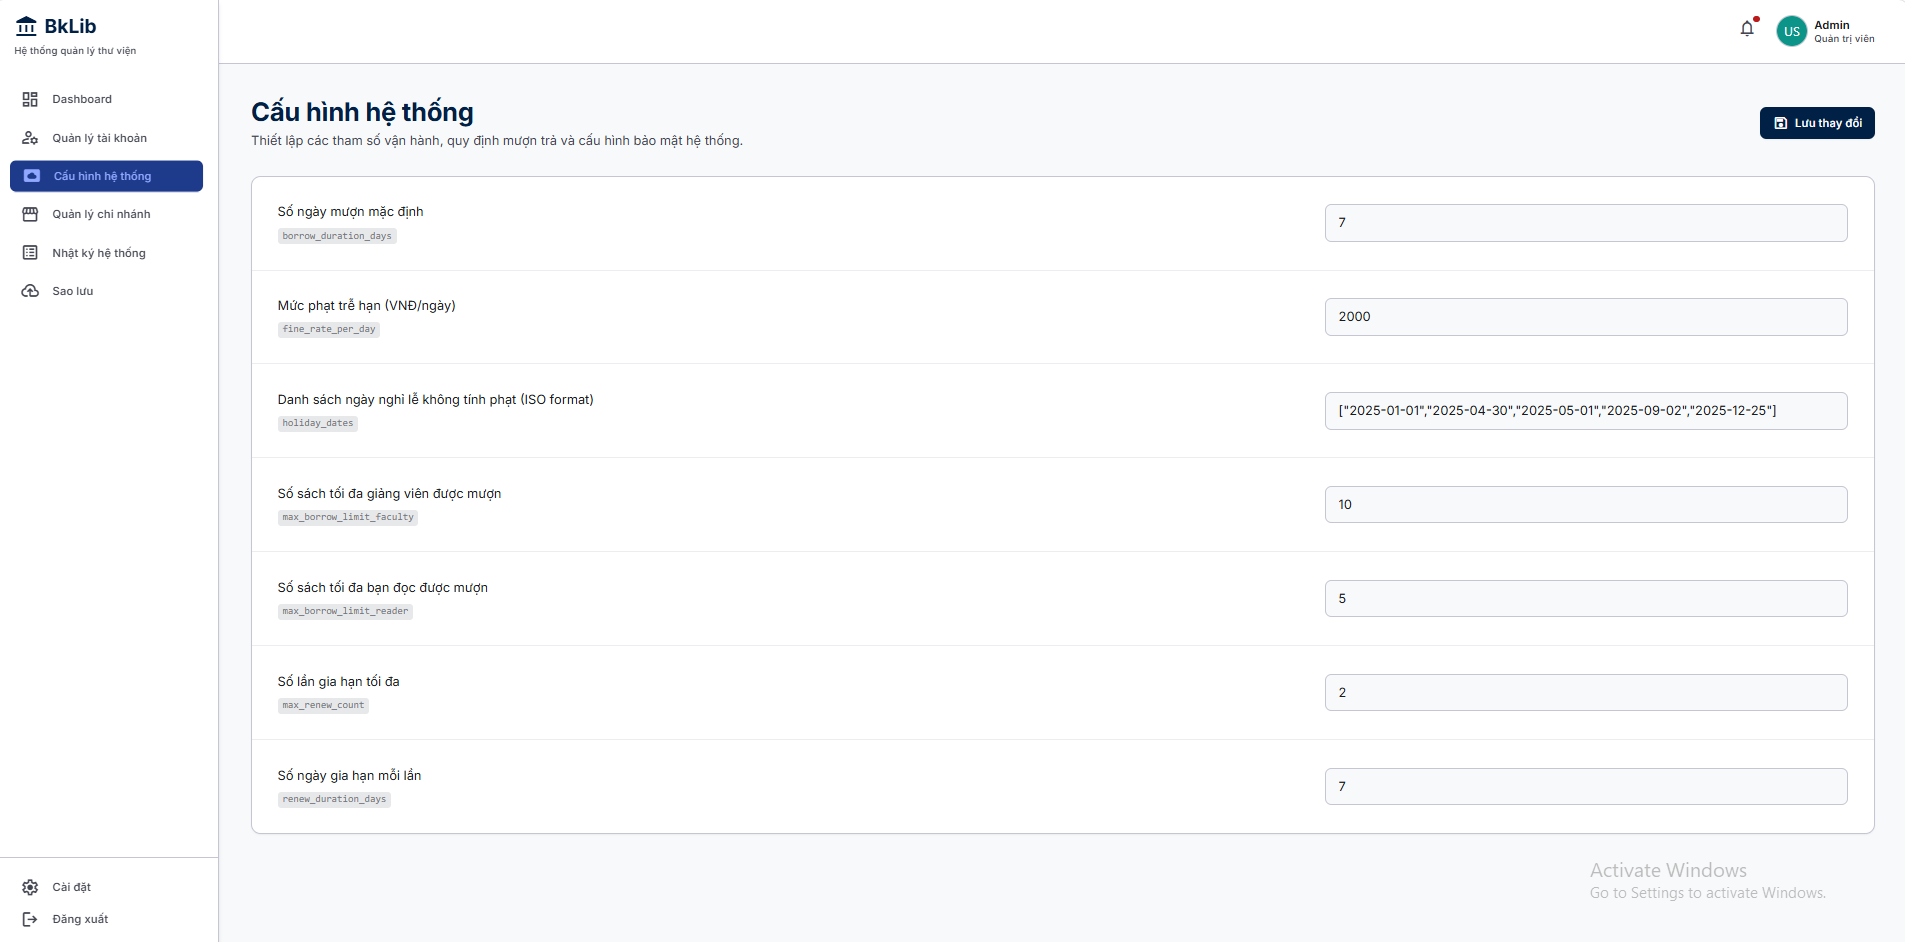
\includegraphics[width=0.95\linewidth]{Images/Admin_CauHinhHeThong.png}
    \vspace{10pt}
    \caption{Giao diện Cấu hình Hệ thống}
    \label{fig:admin_system_config}
\end{figure}

\textbf{Bố cục \& Chức năng:} Bảng cấu hình có cấu trúc cung cấp các ô nhập liệu tương tác cho các biến môi trường hệ thống toàn cục, bao gồm:
\begin{itemize}
    \item \textbf{Quy tắc Lưu thông:} Thời hạn mượn mặc định tính theo ngày (\texttt{borrow\_duration\_days}), hạn mức mượn tối đa cho giảng viên (\texttt{max\_borrow\_limit\_faculty}) và hạn mức mượn chung cho độc giả (\texttt{max\_borrow\_limit\_reader}).
    \item \textbf{Chính sách Gia hạn:} Số lần gia hạn tối đa cho phép (\texttt{max\_renew\_count}) và số ngày kéo dài cho mỗi lần gia hạn (\texttt{renew\_duration\_days}).
    \item \textbf{Cài đặt Tài chính \& Lịch:} Mức phí phạt quá hạn hằng ngày tính theo VNĐ (\texttt{fine\_rate\_per\_day}) và danh sách các ngày nghỉ lễ (\texttt{holiday\_dates}) định dạng ISO để tạm dừng tính phạt trong các ngày nghỉ.
\end{itemize}

\paragraph{Trang Quản lý Chi nhánh}
Trang cấu hình mạng lưới chi nhánh thư viện vật lý và chính sách chuyển sách liên chi nhánh.

\begin{figure}[H]
    \centering
    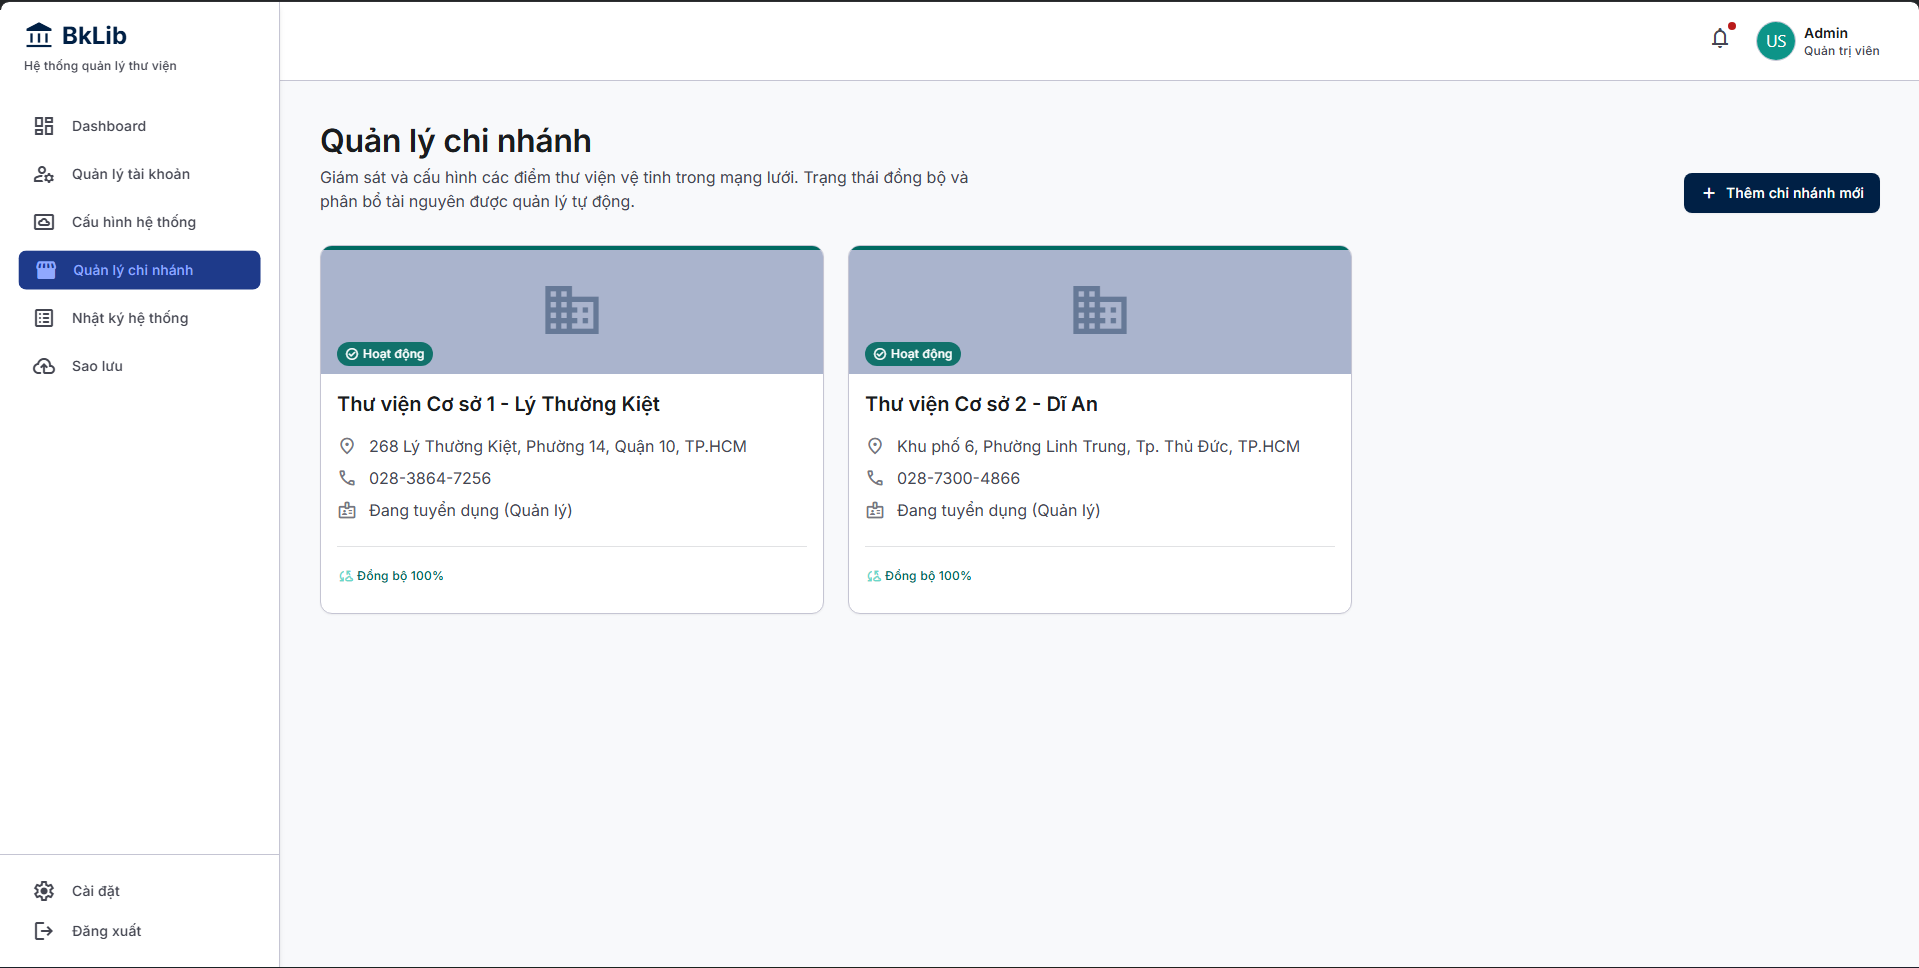
\includegraphics[width=0.95\linewidth]{Images/Admin_QuanLyChiNhanh.png}
    \vspace{10pt}
    \caption{Giao diện Quản lý Chi nhánh}
    \label{fig:admin_branch_management}
\end{figure}

\textbf{Bố cục \& Chức năng:} Lưới các thẻ thông tin chi nhánh hiển thị địa chỉ, chi tiết liên hệ, thủ thư trưởng được phân công, giờ mở cửa và trạng thái đồng bộ với cơ sở dữ liệu trung tâm.

\paragraph{Trang Nhật ký Kiểm toán}
Trình xem nhật ký kiểm toán an ninh ghi lại các hành động quan trọng và các thay đổi trạng thái dữ liệu.

\begin{figure}[H]
    \centering
    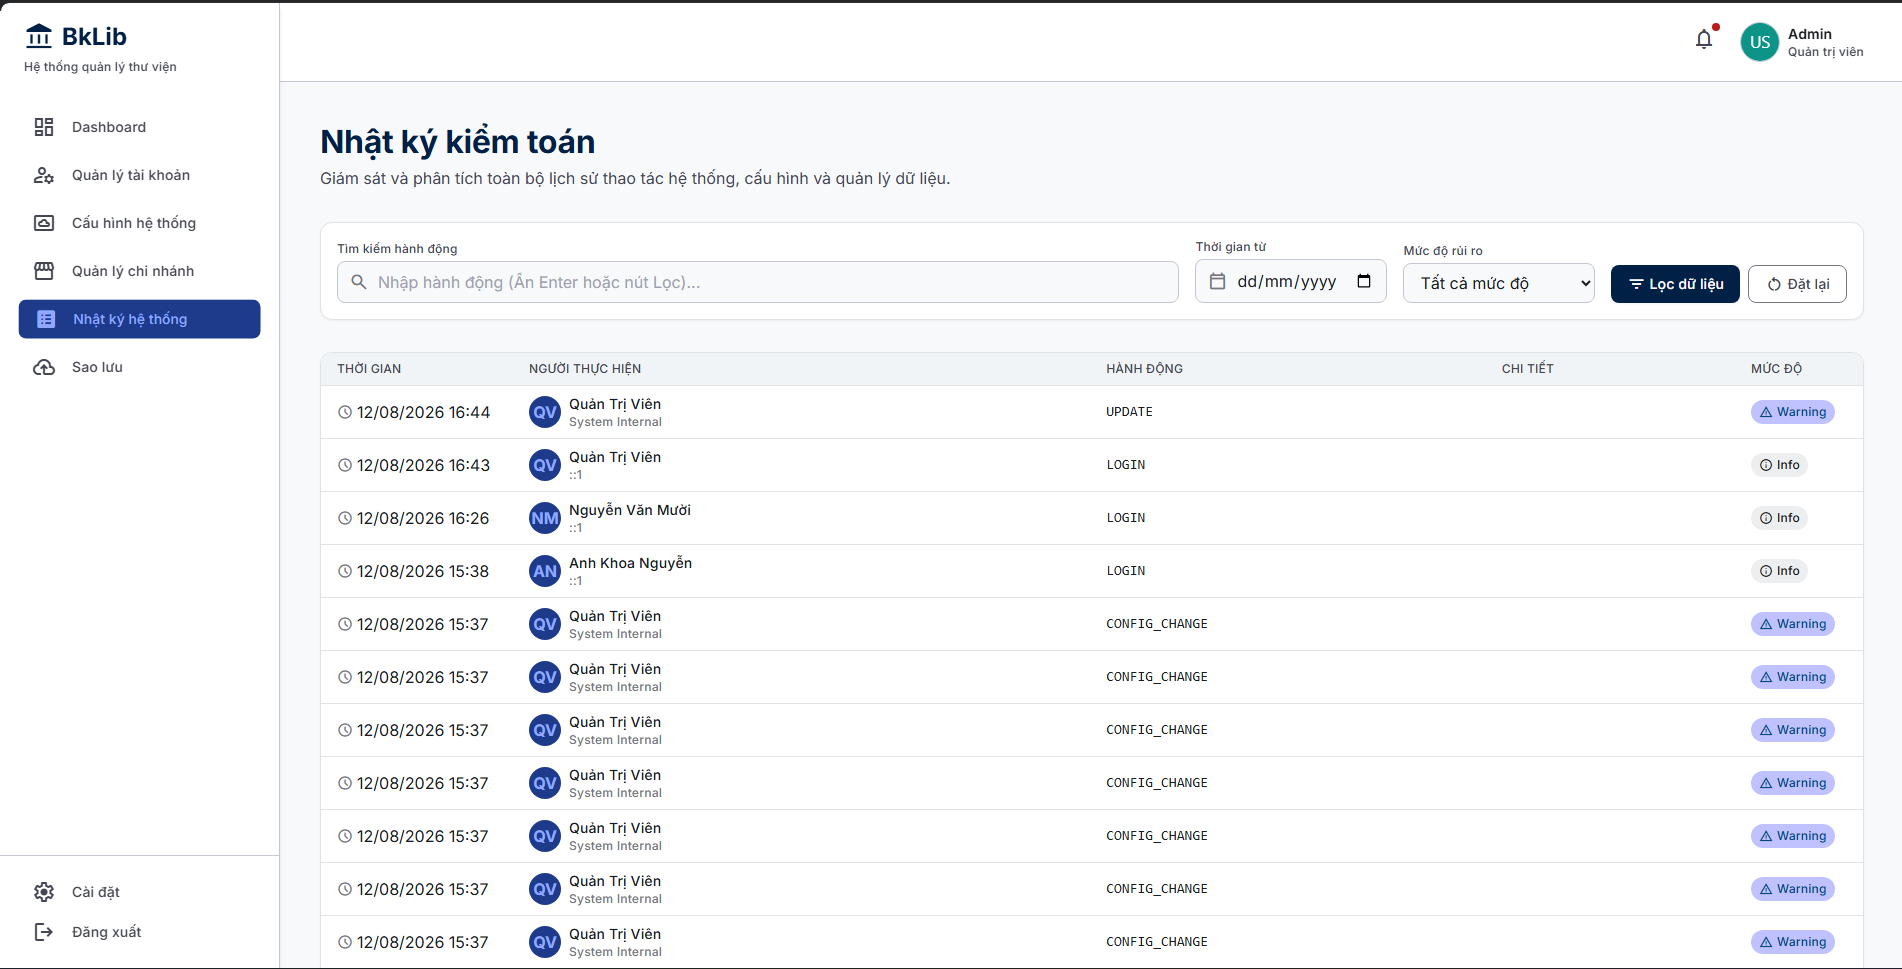
\includegraphics[width=0.95\linewidth]{Images/Admin_NhatKyKiemToan.png}
    \vspace{10pt}
    \caption{Giao diện Nhật ký Kiểm toán Hệ thống}
    \label{fig:admin_audit_log}
\end{figure}

\textbf{Bố cục \& Chức năng:} Bảng sự kiện kiểm toán hiển thị mốc thời gian hành động, danh tính người thực hiện và địa chỉ IP, đường dẫn điểm cuối API, khác biệt dữ liệu JSON trước/sau và huy hiệu mức độ nghiêm trọng để theo dõi bất thường.

\paragraph{Trang Sao lưu \& Phục hồi Dữ liệu}
Công cụ quản lý các bản sao lưu cơ sở dữ liệu và khôi phục sự cố.

\begin{figure}[H]
    \centering
    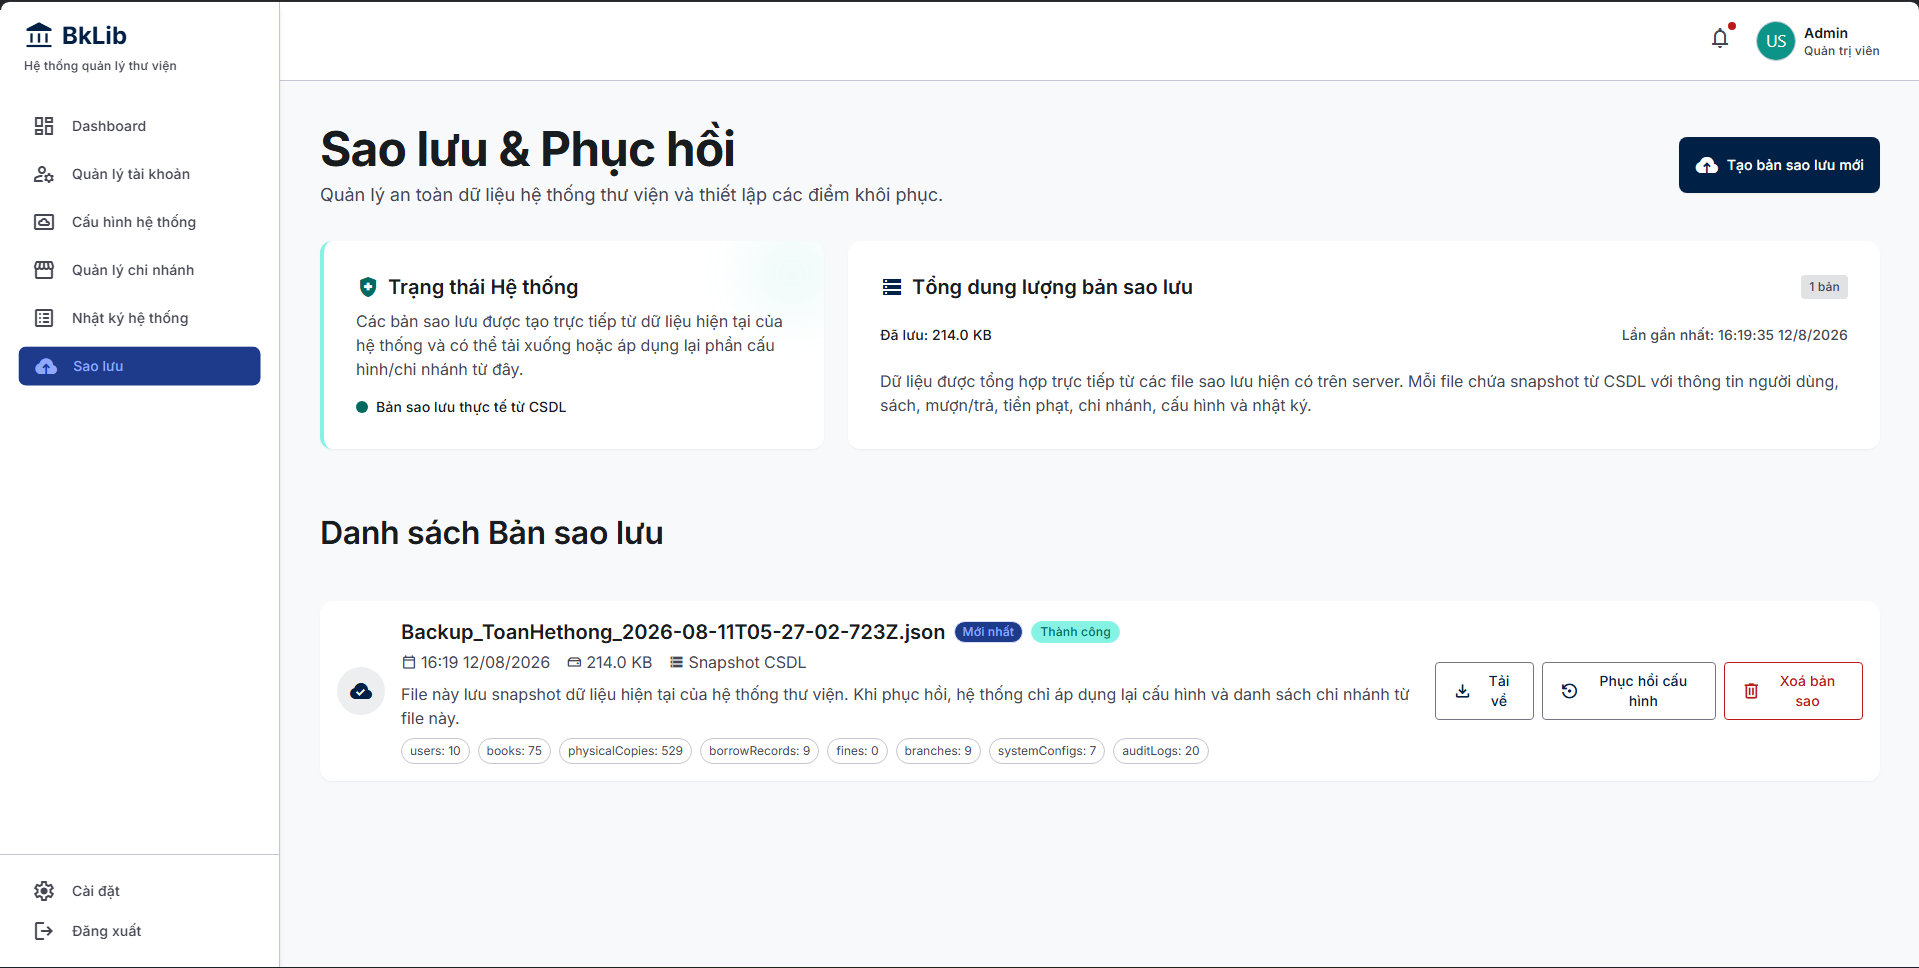
\includegraphics[width=0.95\linewidth]{Images/Admin_SaoLuuPhucHoi.png}
    \vspace{10pt}
    \caption{Giao diện Sao lưu và Phục hồi Dữ liệu}
    \label{fig:admin_backup}
\end{figure}

\textbf{Bố cục \& Chức năng:} Hiển thị cấu hình lịch sao lưu tự động, dung lượng lưu trữ bản sao, nút kích hoạt sao lưu ngay tức thì, nhật ký các bản sao lưu lịch sử và công cụ khôi phục cơ sở dữ liệu về một mốc thời gian cụ thể.

\subsubsection{Các Điểm sáng Hiện thực Kỹ thuật}

Các thao tác quản trị làm thay đổi dữ liệu (như điều chỉnh cấu hình hệ thống, sao lưu cơ sở dữ liệu hay cập nhật tài khoản) tự động ghi lại các bản ghi kiểm toán bất biến chứa dữ liệu người thực hiện và các tham số hành động.

\begin{lstlisting}[caption={Ghi Nhật ký Kiểm toán (backend-express/src/modules/admin/admin.service.ts)}, label={lst:audit_log}]
await prisma.auditLog.create({
  data: {
    actorId: processedById,
    action: AuditAction.SYSTEM_CONFIG_UPDATE,
    targetResource: 'SystemConfig',
    details: { key, oldValue, newValue },
    ipAddress,
  },
});
\end{lstlisting}

% =========================================================================
% SECTION 5.6: DEPLOYMENT STAGE
% =========================================================================
\subsection{Giai đoạn Triển khai}

Phần này mô tả chiến lược triển khai và thiết lập hạ tầng cho hệ thống. Hệ thống được phân phối trên các nhà cung cấp dịch vụ đám mây khác nhau nhằm tận dụng tối đa thế mạnh riêng của từng nền tảng: Vercel được sử dụng cho giao diện frontend và backend Express nhờ khả năng tích hợp CI/CD mượt mà và kiến trúc serverless, trong khi Google Cloud Run được sử dụng cho dịch vụ AI để xử lý hiệu quả các tác vụ máy học được đóng gói dạng container.

\subsubsection{Triển khai Frontend}
Ứng dụng frontend, được xây dựng bằng React và Vite, được triển khai trên Vercel. Vercel cung cấp Mạng lưới Edge Toàn cầu (Edge Network) đảm bảo phân phối nội dung nhanh chóng và tính khả dụng cao. Quy trình triển khai được tích hợp trực tiếp với kho lưu trữ GitHub. Mỗi khi có thao tác push lên nhánh chính (main branch), Vercel sẽ tự động kích hoạt quy trình build mới, thực thi kịch bản biên dịch sản phẩm (production build) và cập nhật trang web trực tuyến. Các biến môi trường, chẳng hạn như URL API backend, được quản lý an toàn trong bảng điều khiển Vercel.

\subsubsection{Triển khai Backend}
Dịch vụ backend, được xây dựng với Node.js và Express, cũng được triển khai trên Vercel bằng cách sử dụng các Hàm Serverless (Serverless Functions). Tiếp cận này loại bỏ nhu cầu tự quản trị máy chủ thủ công và tự động mở rộng quy mô dựa trên lưu lượng truy cập thực tế.
Để cấu hình triển khai, tệp \texttt{vercel.json} được sử dụng tại thư mục gốc của backend để chỉ định môi trường build và các quy tắc định tuyến. Cấu hình điều hướng tất cả các yêu cầu API đến điểm đầu vào chính \texttt{src/app.ts}, sử dụng môi trường thực thi \texttt{@vercel/node}:

\begin{verbatim}
{
  "version": 2,
  "builds": [
    {
      "src": "src/app.ts",
      "use": "@vercel/node"
    }
  ],
  "routes": [
    {
      "src": "/(.*)",
      "dest": "src/app.ts"
    }
  ]
}
\end{verbatim}
Cấu hình này cho phép việc định tuyến của Express hoạt động mượt mà trong môi trường serverless.

\subsubsection{Triển khai Dịch vụ AI}
Dịch vụ AI, chịu trách nhiệm xử lý các tác vụ tiêu tốn tài nguyên như xử lý ngôn ngữ tự nhiên và tìm kiếm ngữ nghĩa, được phát triển bằng Python. Dịch vụ này yêu cầu môi trường thực thi riêng biệt với các phụ thuộc phức tạp được định nghĩa trong \texttt{requirements.txt}. Để đảm bảo tính nhất quán giữa các môi trường, dịch vụ được đóng gói bằng Docker và triển khai lên Google Cloud Run.

\begin{itemize}
    \item \textbf{Đóng gói Container:} Tệp \texttt{Dockerfile} được sử dụng để đóng gói ứng dụng Python, các phụ thuộc hệ thống và các gói thư viện Python thành một hình ảnh Docker (Docker image) tiêu chuẩn.
    \item \textbf{Google Cloud Run:} Cloud Run là một nền tảng tính toán được quản lý hoàn toàn, tự động mở rộng quy mô các container không lưu trạng thái. Nền tảng này được lựa chọn cho dịch vụ AI vì có thể cung cấp hiệu quả các tài nguyên CPU và bộ nhớ cần thiết cho các yêu cầu xử lý và tự động thu hẹp về 0 khi không có truy cập, giúp tối ưu hóa chi phí vận hành.
    \item \textbf{Quy trình Triển khai:} Hình ảnh Docker được biên dịch và đẩy lên Google Artifact Registry. Một dịch vụ Cloud Run sau đó được triển khai tham chiếu đến hình ảnh đã tải lên. Dịch vụ được cấu hình an toàn với các biến môi trường cần thiết và được cấp phát đủ tài nguyên để xử lý các tải công việc AI đồng thời.
\end{itemize}

\subsubsection{Tích hợp Hệ thống}
Kiến trúc triển khai độc lập đảm bảo rằng mỗi dịch vụ có thể mở rộng quy mô một cách riêng biệt dựa trên tải thực tế. Frontend giao tiếp với backend Express trên Vercel thông qua các RESTful API bảo mật chuẩn HTTPS. Backend Express, đến lượt mình, sẽ chuyển tiếp các yêu cầu AI chuyên biệt đến điểm cuối Google Cloud Run, đóng vai trò như một API gateway. Chiến lược triển khai mô-đun này giúp tăng cường khả năng chịu lỗi, tính dễ bảo trì và khả năng mở rộng của toàn bộ hệ thống.

\endgroup